\section{Numerical Experiments}

In this section, we present 3 sets of classical FELA benchmark problems to assess the performance of the proposed ADMM solver in comparison with two state-of-the-art commercial interior-point solvers, MOSEK and Gurobi.

In each of the following examples, we first describe the problem setup and then present numerical results to assess the accuracy, robustness, and scalability of the proposed ADMM solver in comparison with IPM codes. For both the 2D plane-strain and 3D cases, three benchmark problems are considered: the rigid platen, strip footing, and vertical cut problems. For each benchmark, the computational performance of the proposed ADMM solver is compared with that of commercial interior-point solvers in terms of solution time and accuracy. Adaptive mesh refinement results are also presented to demonstrate the FELA formulation’s ability to capture localized failure mechanisms efficiently. 

\subsection{Experimental setup}

Linear stress elements were used in the comparison of accuracy and speed of the in-house solver and IPM solvers in all three geotechnical problems. We use a structured mesh as test problems to the solvers in the benchmark comparison part, and use an adaptively refined mesh to give better quality solution and to demonstrate the failure pattern.

All CPU code was run on an Intel Core i7-12700H, and all GPU code were run on a NVIDIA RTX A1000. We assume Tresca soil with $c = 1$ on 2D problems, and von Mises soil with $k = 1$ on 3D problems. The GPU implementation was developed using NVIDIA CUDA~12.8 and cuDSS~0.5.0. Its performance was compared with MOSEK~11.0 and Gurobi~12.0.2, which served as the commercial interior-point method baselines. In all experiments, MOSEK and Gurobi were run using their default termination criteria on 14 CPU cores.
%%
%\[
%\mathrm{pfeas} \le \varepsilon_{\mathrm{pfeas}}, 
%\qquad 
%\mathrm{dfeas} \le \varepsilon_{\mathrm{dfeas}},
%\]
%with
%\[
%\varepsilon_{\mathrm{pfeas}} = \varepsilon_{\mathrm{dfeas}} = 10^{-3}.
%\]
%%

\subsection{2D Plane Strain Benchmark Problems}

\subsubsection {Rigid Platen Problem}
\paragraph{Problem setup} In this problem, a block of Tresca soil of size $L\times0.5L$ is subjected to compression between two rigid platens. The interfaces between the platens and the soil are assumed to be fully rough. Symmetric boundary conditions are applied to the left and bottom boundaries, while the right boundary is left free. An illustrative representation of the physical setup is provided in Figure~\ref{fig:2PR_CS}.

The exact solution of the load multiplier for the rigid platen problem considered here, $\beta = 2.42768$, was first given by Salençon~\cite{ daSilva_2020, Salencon}. 



\begin{figure}[htbp]
  \centering
  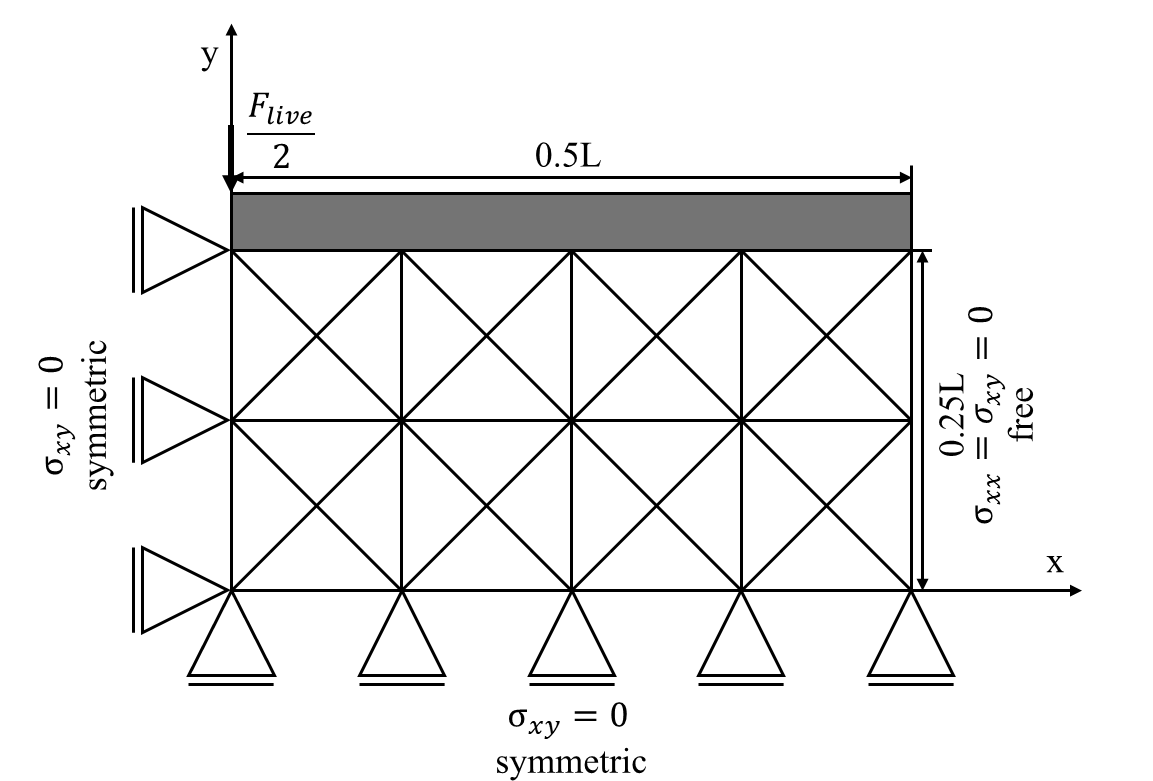
\includegraphics[width=0.50\textwidth]{figures/Res_To_Date/2PR_config.png}
  \hfill
  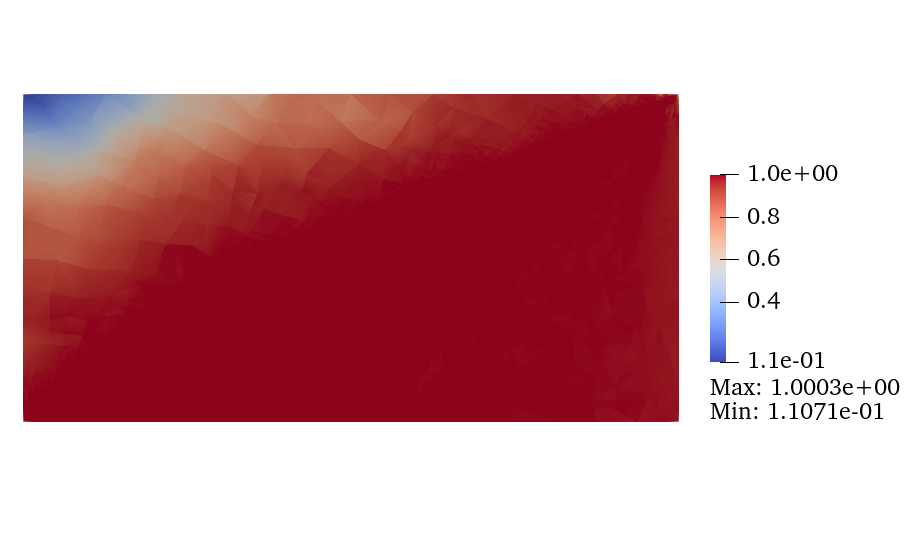
\includegraphics[width=0.46\textwidth]{figures/Res_To_Date/2PR_solution.png}
  \caption{Rigid platen problem. \textbf{Left}: physical configuration; \textbf{Right}: obtained yield function field using AMR with linear stress elements}
  \label{fig:2PR_CS}
\end{figure}

\paragraph{Benchmark comparison using sturctured mesh} 

The proposed ADMM solver is benchmarked against the commercial interior-point solvers MOSEK and Gurobi using structured meshes of linear stress elements with progressively refined discretizations.


\begin{table}[htbp]
\centering
\caption{Solver performance comparison on the 2D rigid platen benchmark for different mesh discretizations}
\label{tab:2PR_timecomp}

\begin{tabular}{@{}C{1.7cm}C{1.7cm}C{1.5cm}C{2.0cm}C{2.3cm}C{2.3cm}C{2.3cm}@{}}
\toprule
\multicolumn{2}{c}{\textbf{Problem size}} &
\textbf{Solver} &
\textbf{Solve time (s)} &
\textbf{Collapse multiplier} &
\textbf{Iterations}&
\textbf{Time-per-iter (s)}
\tabularnewline
\cmidrule(lr){1-2}
\textbf{$N_{\mathrm{elem}}(\times 10^3)$} &
\textbf{$N_{\mathrm{var}}(\times 10^6)$} &
&
&
&
\tabularnewline
\midrule

\multirow{3}{*}{20.0}
& \multirow{3}{*}{0.18}
& MOSEK  & 8.80 & 2.42465 &  32  &0.37 \tabularnewline
& & Gurobi & 6.96   & 2.42465&   26    & 0.28 \tabularnewline
& & ADMM   & 2.66 & 2.42467&  340  & 0.0078 \tabularnewline

\addlinespace

\multirow{3}{*}{28.8}
& \multirow{3}{*}{0.26}
& MOSEK  & 31.75 & 2.42514 &  35  &0.91 \tabularnewline
& & Gurobi & 13.98    & 2.42514 & 30  & 0.68 \tabularnewline
& & ADMM   & 3.62  & 2.42516& 260 & 0.014 \tabularnewline

\addlinespace

\multirow{3}{*}{51.2}
& \multirow{3}{*}{0.46}
& MOSEK  & 60.03 & 2.42576 & 46 & 1.11 \tabularnewline
& & Gurobi & 27.60    & 2.42577 & 34 & 1.31 \tabularnewline
& & ADMM   & 5.74  & 2.42577& 300 & 0.019 \tabularnewline

\addlinespace

\multirow{3}{*}{80.0}
& \multirow{3}{*}{0.72}
& MOSEK  & 43.14 & 2.42614 & 38 & 1.14 \tabularnewline
& & Gurobi & 50.81    & 2.42614   & 27   & 2.48 \tabularnewline
& & ADMM   & 9.82  & 2.42611 & 340 & 0.029 \tabularnewline

\addlinespace

\multirow{3}{*}{204.8}
& \multirow{3}{*}{1.84}
& MOSEK  & 95.24 & 2.42669 & 39 & 3.024 \tabularnewline
& & Gurobi & 342.17    & 2.42671  &  32  & 12.01 \tabularnewline
& & ADMM   & 20.36 & 2.42669&  280  & 0.073 \tabularnewline

\bottomrule
\end{tabular}

\vspace{0.5em}
\end{table}

Table~\ref{tab:2PR_timecomp} shows that the proposed solver delivers superior computational performance, achieving a speedup of \(4\times\) to \(10\times\) over the state-of-the-art IPM solvers, while maintaining high solution accuracy in all cases. For each mesh discretization, all three solvers converge to closely comparable collapse multipliers. The problem sizes are reported in Table~\ref{tab:2PR_timecomp}, ranging from 0.18 million variables to 1.84 million variables. 


The computed collapse multipliers remain below the analytical solution reported by Salen\c{c}on~\cite{daSilva_2020, Salencon}. This gap is primarily due to the use of a structured mesh. Using higher-order stress elements may mitigate this effect and yield a tighter lower bound. We nonetheless adopt structured meshes in this example to ensure controlled and consistent problem generation, which is desirable for a fair performance comparison. Overall, the results reported here demonstrated that the proposed ADMM methodology works well on these types of PDE-constrained optimization problem.


\paragraph{Adaptive mesh refinement solution}

Using AMR, we obtain a tighter lower bound solution of $\beta = 2.426787$ using linear stress elements, together with AMR, the resulting yield function is shown in Figure~\ref{fig:2PR_CS}, with the final adaptively refined mesh after 10 refinements shown in Figure~\ref{fig:2PR_mesh}. This gives a relative error of only 0.036\%, the refined mesh concentrated around the yielded area. Moreover, the zone that had been refined the most agrees well with the solutions of da Silva~\cite{daSilva_2020} and with the classical slip line solutions~\cite{Slip_Line_Hosford}.

\begin{figure}
\centering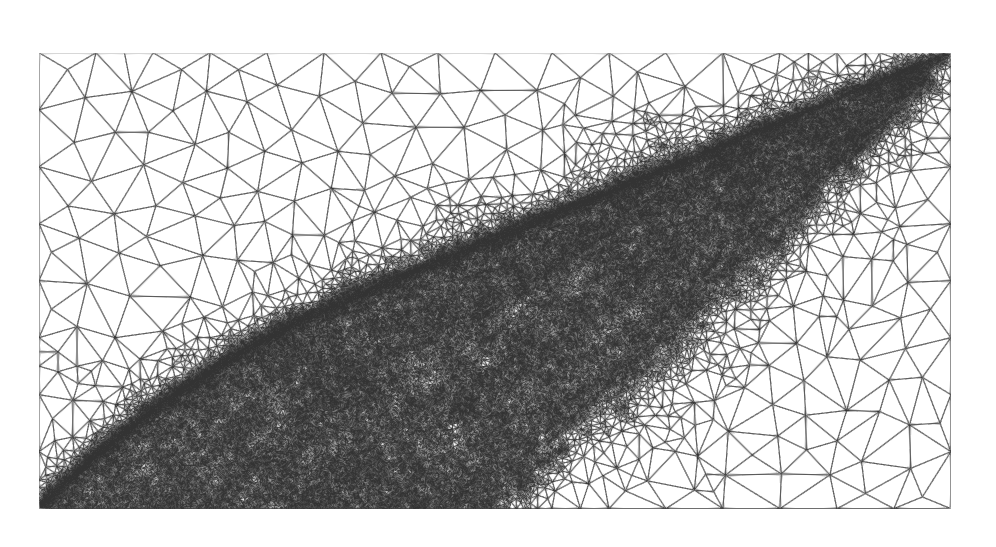
\includegraphics[width=0.8\textwidth]{figures/Res_To_Date/2PR_mesh.png} 
\caption[AMR result of the rigid platen problem]{AMR result of the rigid platen problem}
\label{fig:2PR_mesh}
\end{figure}



\subsubsection{Strip Footing Problem}
\paragraph{Problem setup}
An illustrative representation of the problem is shown in Figure~\ref{fig:SF_CS}. Here, a rigid body is placed at the upper-left corner of the domain to represent a strip footing. A fixed boundary condition is applied on the right and bottom edges, and a symmetric boundary condition on the left edge. The fixed boundaries are sufficiently far from the footing to have a minimal effect  on the result.


The ultimate bearing capacity of a strip footing on weightless cohesive soil is a foundational result in geotechnical engineering. The exact solution of the load multiplier to this problem is $\beta = 2+\pi$, a result first derived by Prandtl~\cite{ Sloan_stability_analysis, 2DLB, Prandtl}. Martin developed software ABC for calculating the ultimate bearing capacity of this footing using the method of characteristics~\cite{Slip_Line_2005}. A FELA-based solution to this problem with adaptive mesh refinement was first given by Lyamin~\cite{adaptive_mesh_Lyamin}, demonstrating that the approach can deliver accurate collapse loads while systematically assessing a range of adaptive remeshing strategies.


\begin{figure}[htbp]
  \centering
  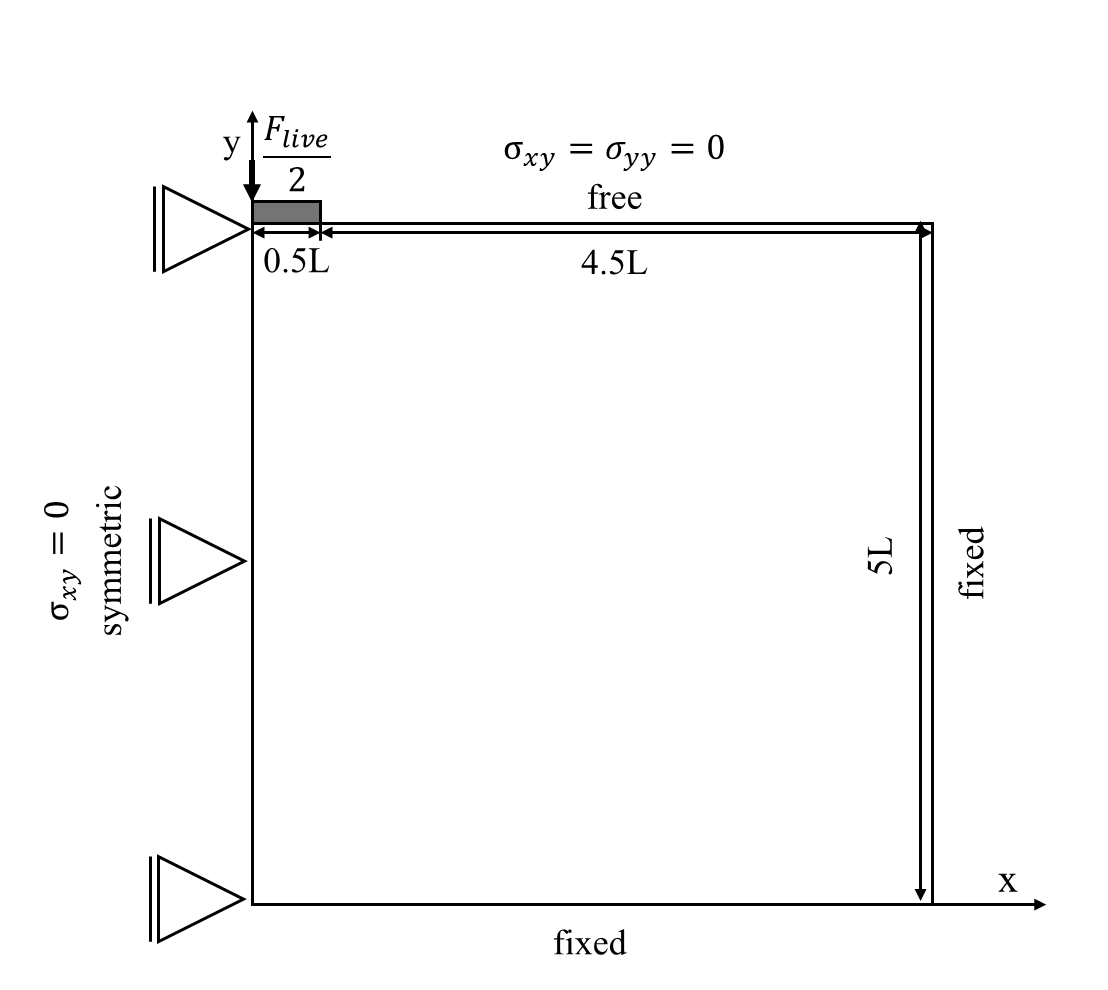
\includegraphics[width=0.50\textwidth]{figures/Res_To_Date/SF_config.png}
  \hfill
  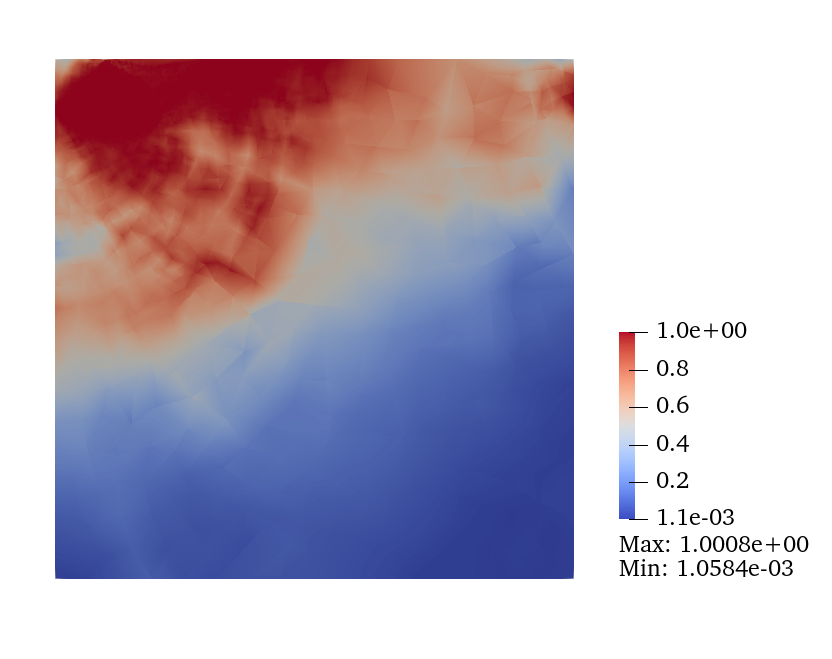
\includegraphics[width=0.47\textwidth]{figures/Res_To_Date/SF_solution.png}
  \caption{Strip footing problem. \textbf{Left}: physical configuration; \textbf{Right}: solution of the yield function using AMR and linear stress elements}
  \label{fig:SF_CS}
\end{figure}

\paragraph{Benchmark comparison using structured mesh} We first demonstrate the performance of our 2D condensed-form ADMM solver on different mesh discretizations, all using linear stress elements. 



\begin{table}[htbp]
\centering
\caption{Solver performance comparison on the 2D strip footing benchmark for different mesh discretization}
\label{tab:SF_detail}

\begin{tabular}{@{}C{1.7cm}C{1.7cm}C{1.5cm}C{2.0cm}C{2.3cm}C{2.3cm}C{2.3cm}@{}}
\toprule
\multicolumn{2}{c}{\textbf{Problem size}} &
\textbf{Solver} &
\textbf{Solve time (s)} &
\textbf{Collapse multiplier} &
\textbf{Iterations}&
\textbf{Time-per-iter (s)}
\tabularnewline
\cmidrule(lr){1-2}
\textbf{$N_{\mathrm{elem}}(\times 10^3)$} &
\textbf{$N_{\mathrm{var}}(\times 10^6)$} &
&
&
&
\tabularnewline
\midrule

\multirow{3}{*}{40.0}
& \multirow{3}{*}{0.36}
& MOSEK  & 27.37 & 5.09752 &  32  &0.86 \tabularnewline
& & Gurobi & 24.73   & 5.09753&   231    & 1.09 \tabularnewline
& & ADMM   & 6.08 & 5.09768&  440  & 0.014 \tabularnewline

\addlinespace

\multirow{3}{*}{57.6}
& \multirow{3}{*}{0.52}
& MOSEK  & 48.59 & 5.10470 &  38  & 1.28 \tabularnewline
& & Gurobi & 26.78    & 5.10470 & 27  & 1.26 \tabularnewline
& & ADMM   & 8.47  & 5.10482& 440 & 0.019 \tabularnewline

\addlinespace

\multirow{3}{*}{102.4}
& \multirow{3}{*}{0.92}
& MOSEK  & 204.05 & 5.11383 & 50 & 5.57 \tabularnewline
& & Gurobi & 173.61    & 5.11383 & 35 & 4.08 \tabularnewline
& & ADMM   & 13.77  & 5.11392 & 400 & 0.034 \tabularnewline

\addlinespace

\multirow{3}{*}{160.0}
& \multirow{3}{*}{1.44}
& MOSEK  & 126.85 & 5.11932 & 33 & 3.84 \tabularnewline
& & Gurobi & 270.60    & 5.11932   & 35   & 8.59 \tabularnewline
& & ADMM   & 25.82  & 5.11939 & 460 & 0.056 \tabularnewline

\bottomrule
\end{tabular}

\vspace{0.5em}
\end{table}

Table~\ref{tab:SF_detail} shows that the proposed GPU-based ADMM solver remains faster than the CPU-parallelized IPM solver MOSEK and Gurobi, while producing almost identical collapse multipliers. The observed speedup ranges from $3.12\times$ to $5.7\times$ for MOSEK, and $6.04\times$ to $17.28\times$ for Gurobi. Although this improvement is less pronounced than that obtained for the 2D rigid platen problem, it still demonstrates the efficiency of the proposed solver on classical FELA problems.

The final load multiplier remains below Prandtl's analytical solution of $2+\pi$, with an error of only $0.27\%$. This discrepancy is mainly due to the use of linear stress elements on structured meshes for benchmarking. A tighter LB solution is obtained below using AMR and linear stress elements:

\paragraph{Adaptive mesh refinement solution} Here we demonstrate an ADMM–FELA framework enhanced by AMR using linear stress elements. By mapping the solution from the previous mesh onto the refined mesh as the initial iterate, we achieve a substantial reduction in iterations while maintaining accuracy. The final yield function field, after 9 refinements, is given in Figure~\ref{fig:SF_CS}. Solving this problem yields a load multiplier of $\beta = 5.13648$, while only using 58.5 seconds in its final iteration. The obtained load multiplier agrees well with the analytical solution by Prandtl~\cite{Prandtl, 2DLB}.

\begin{figure}[htbp]
  \centering
  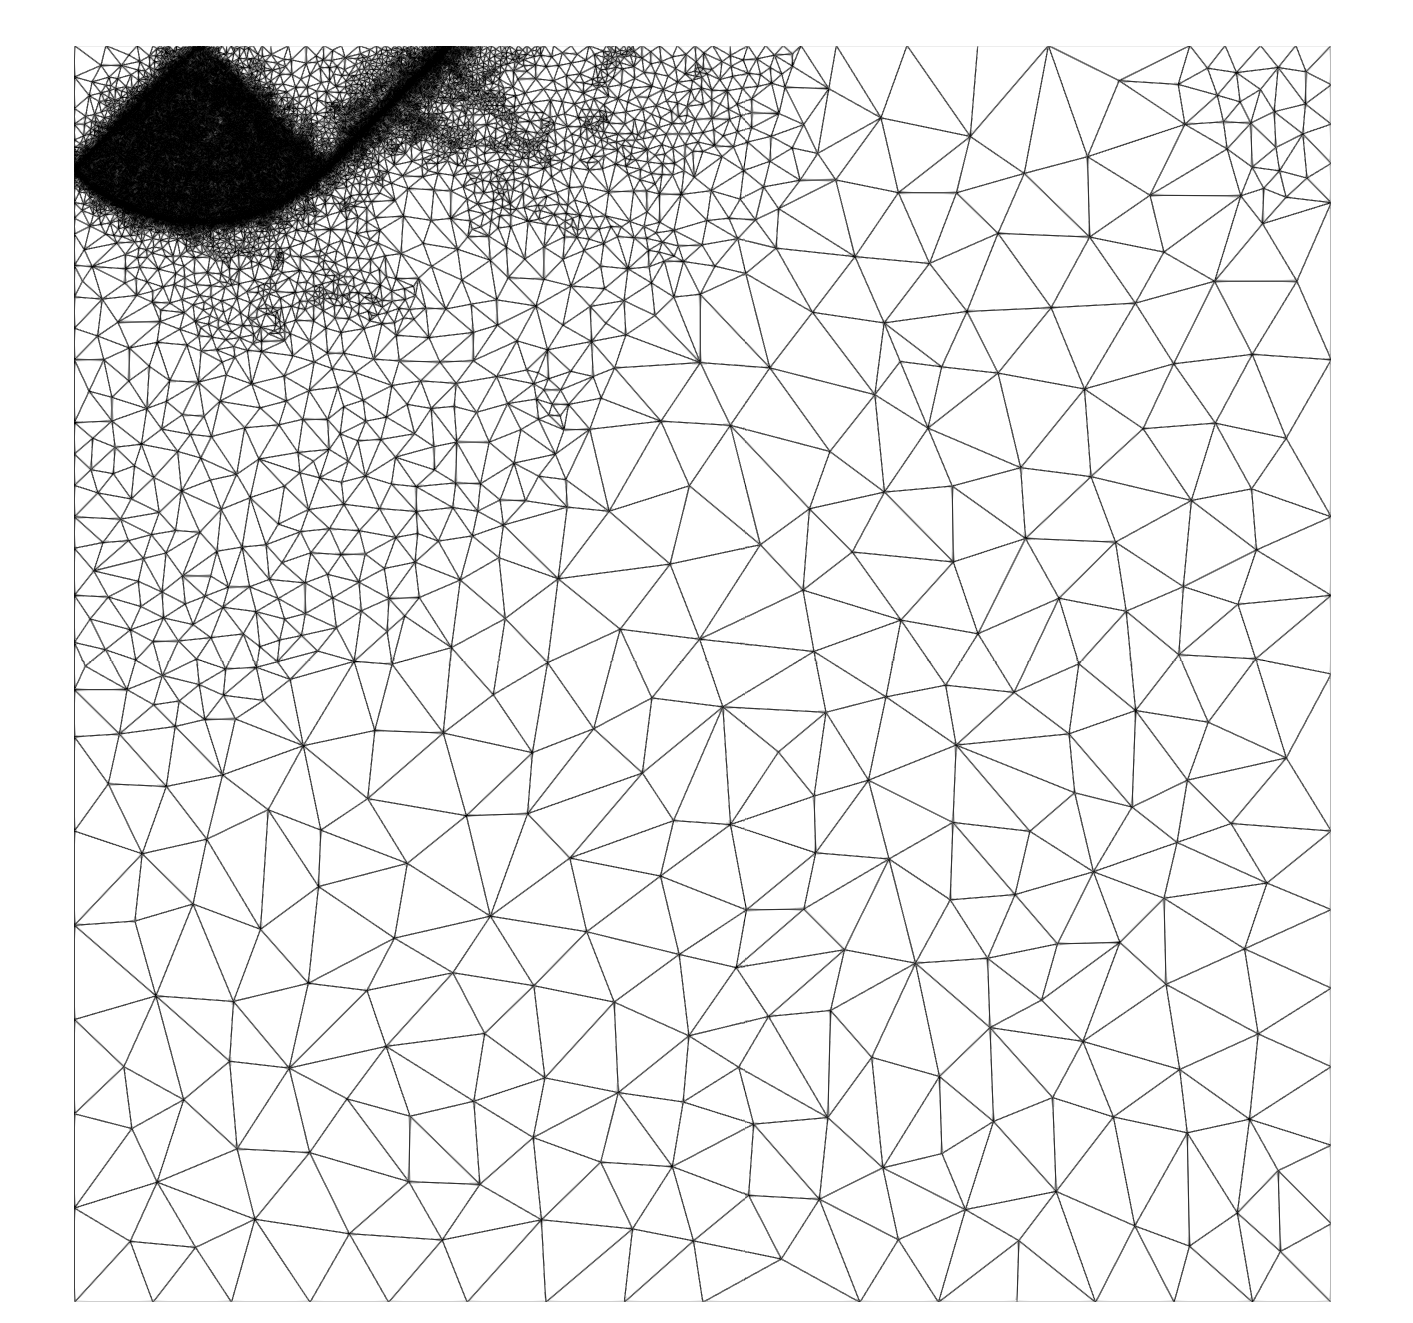
\includegraphics[width=0.37\textwidth]{figures/Res_To_Date/SF_mesh.png}
  \hfill
  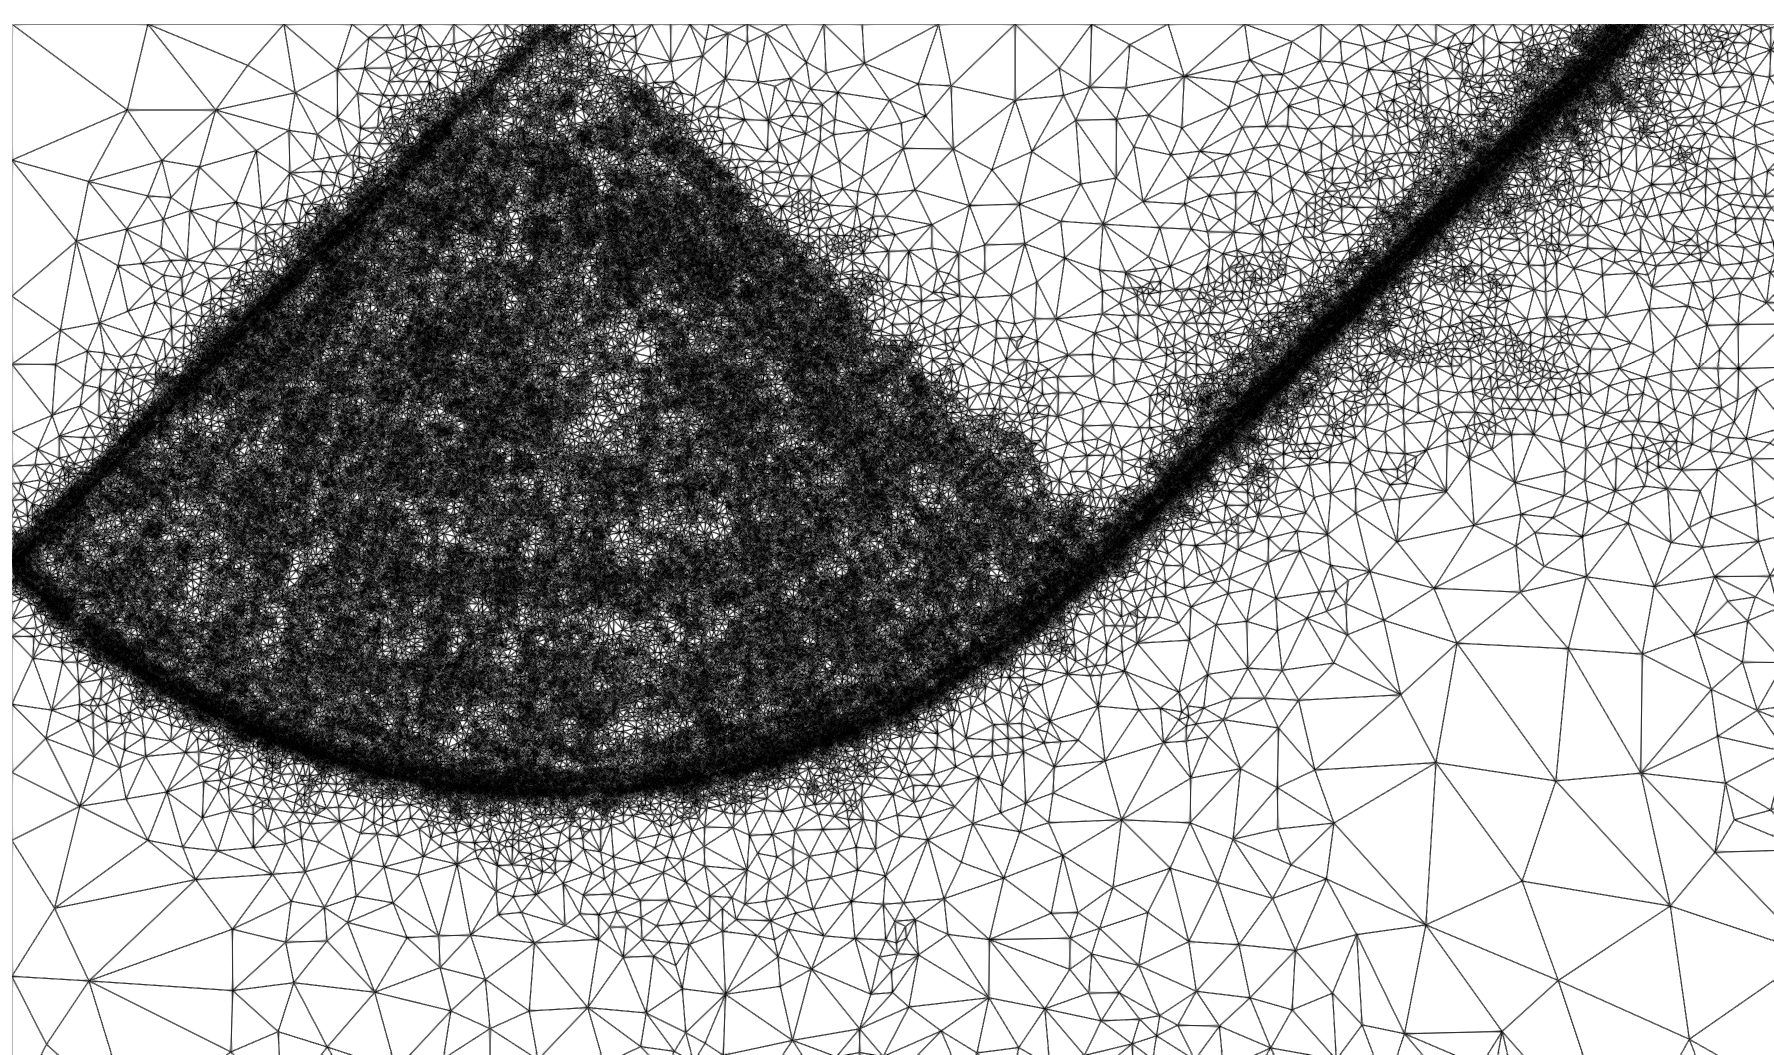
\includegraphics[width=0.59\textwidth]{figures/Res_To_Date/SF_mesh_slip_line.png}
  \caption{AMR mesh of the strip footing problem in plane strain. \textbf{Left}: overall obtained mesh; \textbf{Right}: zoomed view highlighting the refined area}
  \label{fig:SF_Mesh}
\end{figure}
The resulting AMR mesh shown in Figure~\ref{fig:SF_Mesh} is consistent with the sequential limit-analysis meshes reported by Kong~\cite{Kong_2017} and Martin~\cite{Slip_Line_2005, Martin_2011}, in that the refined region correctly matches the slip-line zone. 

This example also highlights the overall efficiency of the proposed solver, which attains rapid convergence on large-scale problems. Our solver converges easier due to exploiting the problem structure by warm-starting each AMR solve with the solution from the previous mesh.


\subsubsection{Vertical Cut Problem}


\paragraph{Problem setup}
We consider a square soil block with a vertical excavation on its left side, subjected to a uniform body force representing a live load. The top surface and the excavated left boundary are assumed to be free, while the right and bottom boundaries are taken as rough and fixed. An illustrative representation of the problem and a numerical solution given by using AMR is shown in Figure~\ref{fig:VC_CS}. This benchmark is of particular interest because the uniform body force introduces a dense column into the matrix $A$, which can pose a challenge for solver performance.

Although, to the best of the authors' knowledge, no analytical solution has been reported in the literature, Martin~\cite{Martin_2011} provided a tight bound on the ultimate bearing capacity, $3.7764904 < N < 3.7764911$, using finite element limit analysis with adaptive mesh refinement. The corresponding slip-line field was also obtained using this approach.

\begin{figure}[htbp]
  \centering
  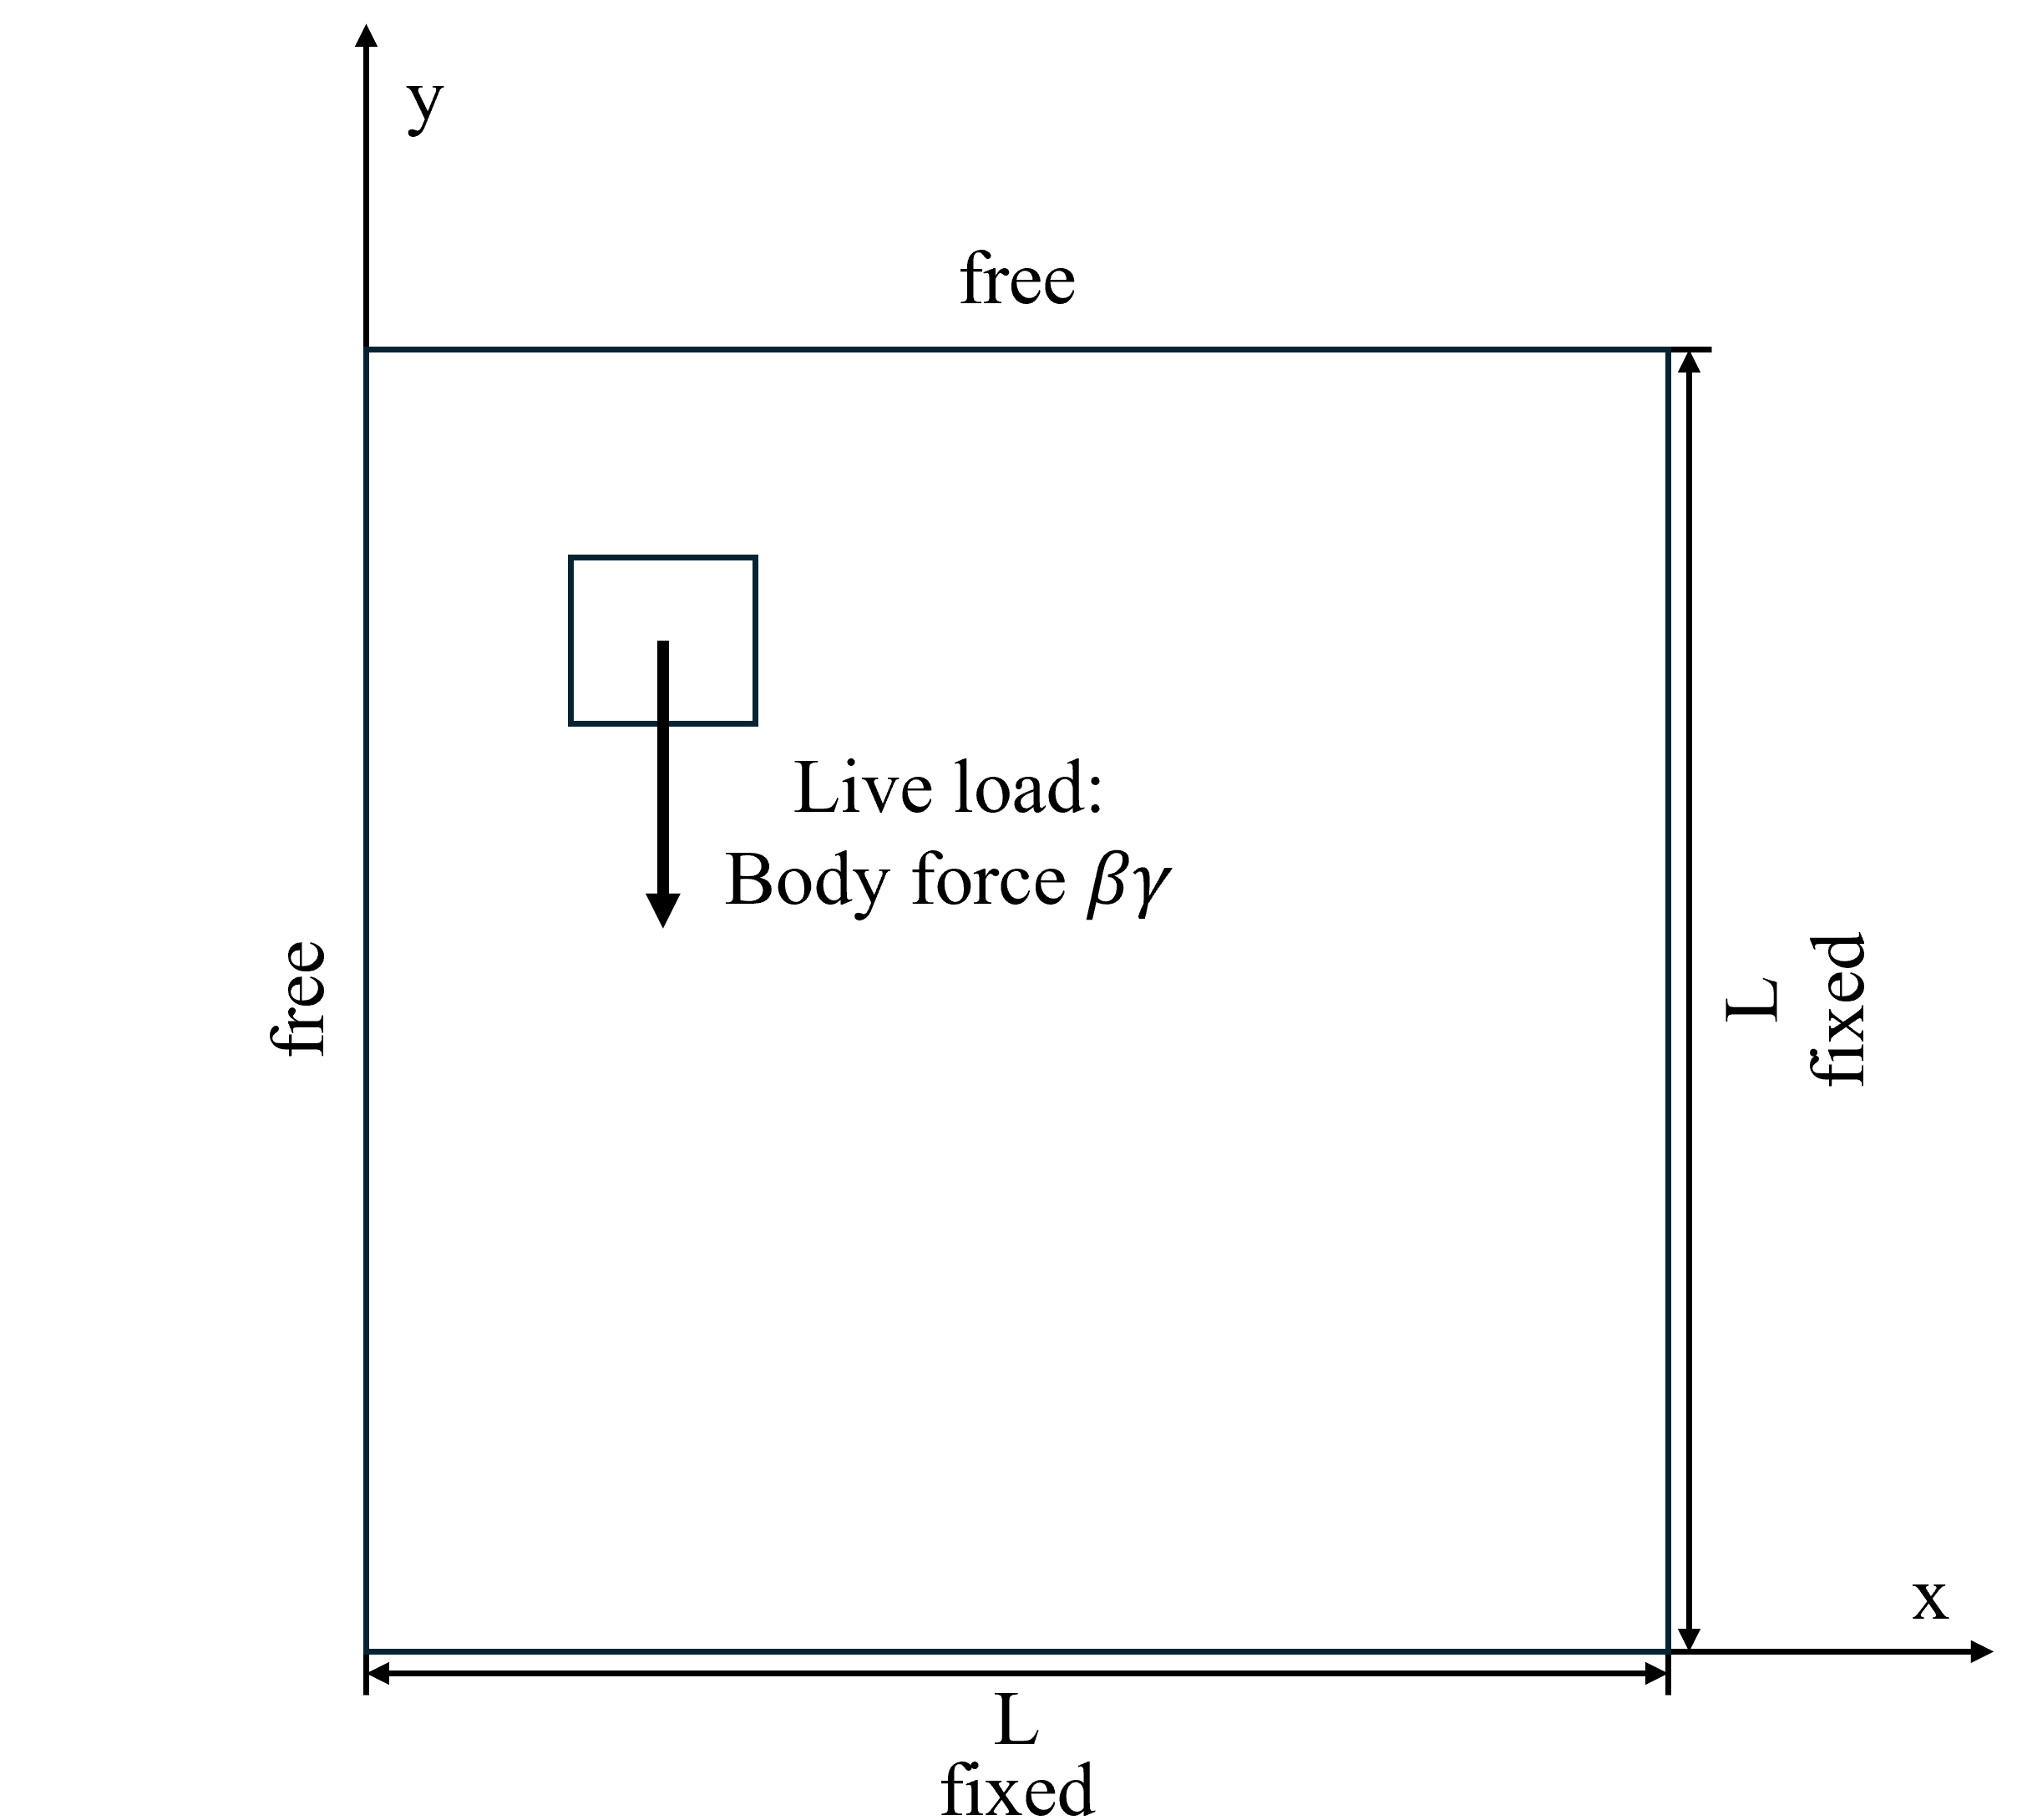
\includegraphics[width=0.48\textwidth]{figures/Res_To_Date/VC_config.png}
  \hfill
  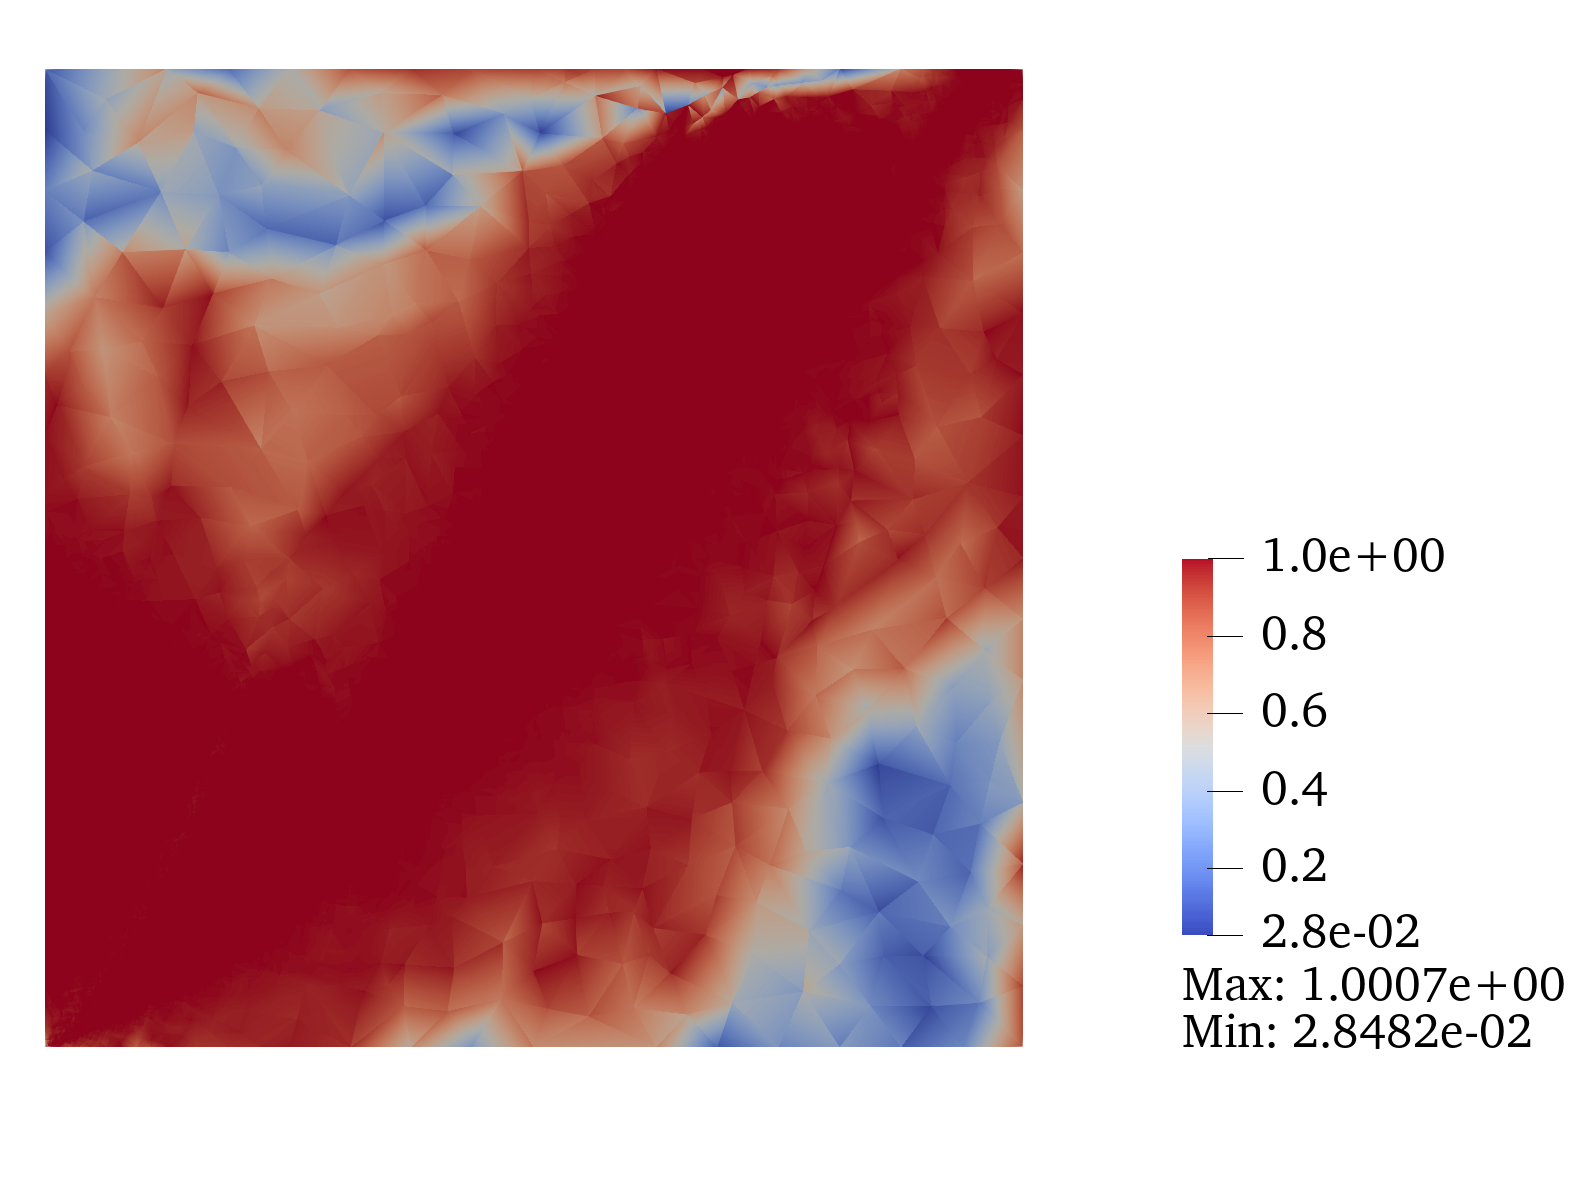
\includegraphics[width=0.48\textwidth]{figures/Res_To_Date/VCSM_SOL.png}
  \caption{Vertical cut problem. \textbf{Left}: physical configuration; \textbf{Right}: obtained yield function field}
  \label{fig:VC_CS}
\end{figure}



\paragraph{Benchmark Comparison using structured mesh}
We first assess the performance of the proposed ADMM solver using a sequence of increasingly refined meshes using linear stress elements. 

As shown in Table~\ref{tab:VC_timecomp}, the proposed ADMM solver constantly outperforms the IPM solvers in problems with dimension ranging from 0.36 to 1.44 million variables. ADMM attained a speedup from 6.6$\times$ to 17.6$\times$ compared with MOSEK, and from 6.0$\times$ to 17.3$\times$ with Gurobi. Even with the improvements made to speed up convergence, the problems still takes around 300 to 500 iterations, but each iteration is considerably cheaper than the IPM iterations. Also, the ADMM solver attained the speedup while preserving accuracy, obtaining a nearly identical load multiplier with the accurate IPM solvers.

\begin{table}[htbp]
\centering
\caption{Solver performance comparison on the 2D vertical cut benchmark for different mesh discretization}
\label{tab:VC_timecomp}

\begin{tabular}{@{}C{1.7cm}C{1.7cm}C{1.5cm}C{2.0cm}C{2.3cm}C{2.3cm}C{2.3cm}@{}}
\toprule
\multicolumn{2}{c}{\textbf{Problem size}} &
\textbf{Solver} &
\textbf{Solve time (s)} &
\textbf{Collapse multiplier} &
\textbf{Iterations}&
\textbf{Time-per-iter (s)}
\tabularnewline
\cmidrule(lr){1-2}
\textbf{$N_{\mathrm{elem}}(\times 10^3)$} &
\textbf{$N_{\mathrm{var}}(\times 10^6)$} &
&
&
&
\tabularnewline
\midrule

\multirow{3}{*}{40.0}
& \multirow{3}{*}{0.36}
& MOSEK  & 42.90 & 3.77269 &  40  &1.12 \tabularnewline
& & Gurobi & 39.27   & 3.77269&   34    & 1.28 \tabularnewline
& & ADMM   & 4.14 & 3.77255&  460  & 0.025 \tabularnewline

\addlinespace

\multirow{3}{*}{57.6}
& \multirow{3}{*}{0.52}
& MOSEK  & 43.08 & 3.77334 &  46  & 1.09 \tabularnewline
& & Gurobi & 57.85    & 3.77333 & 37  & 1.77 \tabularnewline
& & ADMM   & 5.47  & 3.77330 & 340 & 0.035\tabularnewline

\addlinespace

\multirow{3}{*}{102.4}
& \multirow{3}{*}{0.92}
& MOSEK  & 116.40 & 3.77412 & 43 & 3.13 \tabularnewline
& & Gurobi & 164.12    & 3.77413 & 43 & 4.13 \tabularnewline
& & ADMM   & 11.66  & 3.77410 & 320 & 0.071 \tabularnewline

\addlinespace

\multirow{3}{*}{160.0}
& \multirow{3}{*}{1.44}
& MOSEK  & 303.89 & 3.77459 & 50 & 6.66 \tabularnewline
& & Gurobi &  298.47   & 3.77460   & 45   & 7.14 \tabularnewline
& & ADMM   & 17.27  & 3.77458 & 300 & 0.13 \tabularnewline

\bottomrule
\end{tabular}

\vspace{0.5em}
\end{table}



\paragraph{Adaptive Mesh Solution}
With the use of AMR, the best LB estimation we may obtain is 3.775063 using linear stress elements, the adaptive refined mesh is shown in Figure~\ref{fig:VC_AMR}. 

\begin{figure}[htbp]
  \centering
  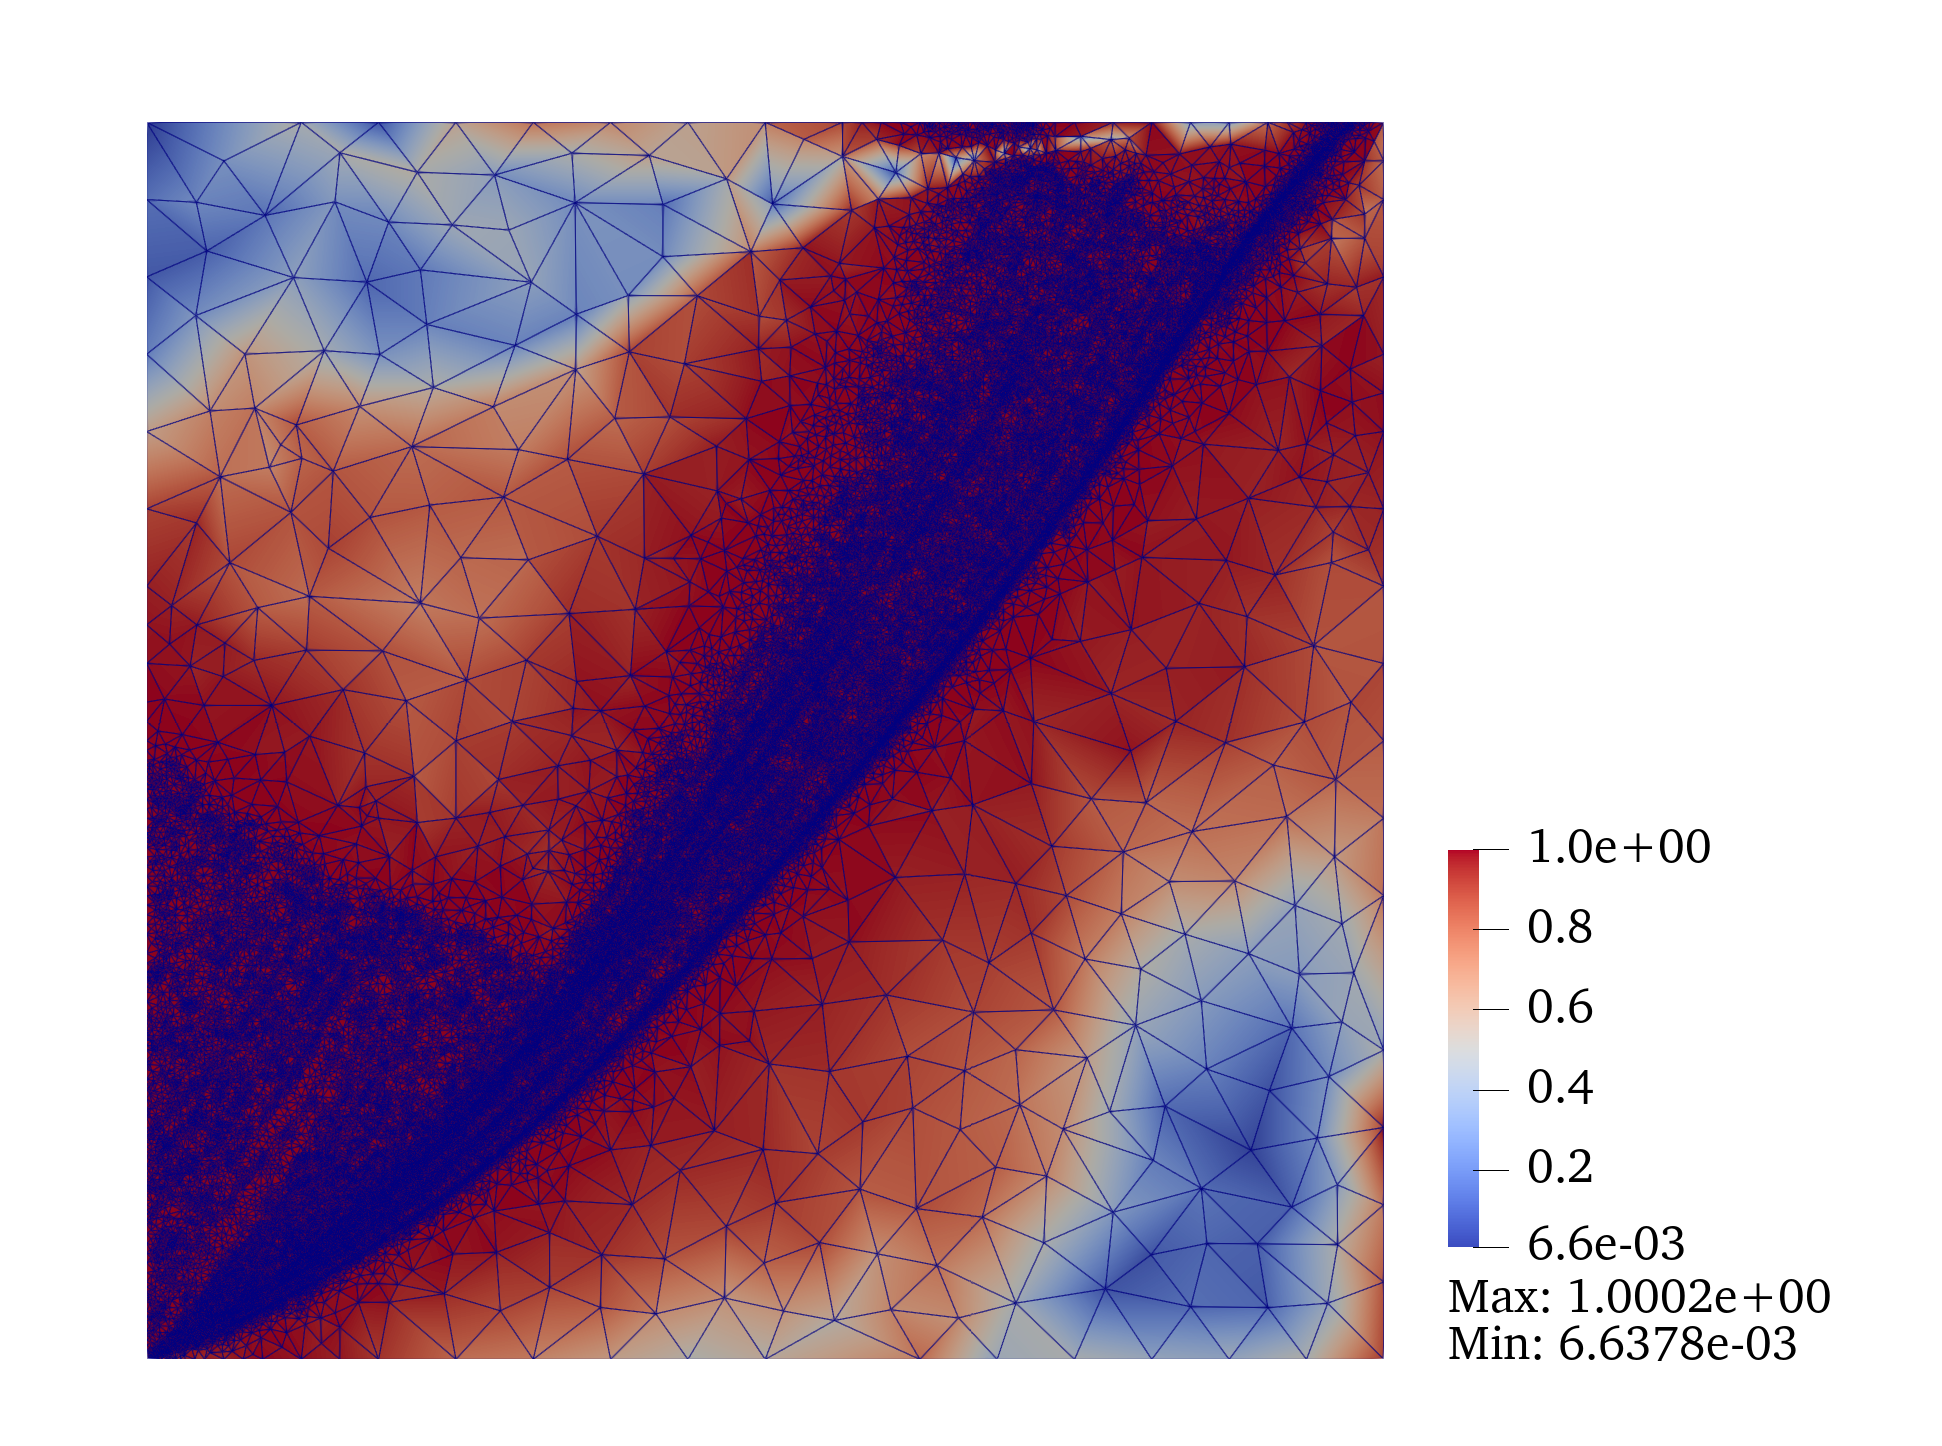
\includegraphics[width=0.9\textwidth]{figures/Res_To_Date/VCSM_Tresca stress.png}
  \caption{AMR mesh of the vertical cut problem in plane strain}
  \label{fig:VC_AMR}
\end{figure}

We may observe from Figure~\ref{fig:VC_AMR} that the refined zone matches with the slip-line zone reported in previous work by Martin~\cite{Martin_2011}. 


\subsubsection{Discussion}

After examining the three 2D benchmark problems individually, we summarize the overall timing performance of the solvers in Figure~\ref{fig:2DTimecomp}. The figure compares the time to solution of ADMM, MOSEK, and Gurobi as the problem size increases for the rigid platen, strip footing, and vertical cut problems. Gurobi is often faster than MOSEK for smaller problem instances, but its performance deteriorates significantly for larger problems. In contrast, the proposed ADMM solver consistently achieves the shortest solution times while maintaining close agreement with the IPM solutions, with the absolute difference in the computed collapse multiplier remaining below approximately $10^{-4}$.  This speedup is primarily attributed to the substantially lower cost per ADMM iteration compared with that of the IPM solvers, together with the fact that the number of ADMM iterations increases only moderately as the problem size grows.





The irregular spikes observed in the MOSEK timings for the rigid platen and strip footing problems are primarily attributed to a larger number of interior-point iterations required for those particular cases.



Specifically, we investigate the individual effects of the two proposed acceleration strategies, namely warm-starting (WS) and active-cone identification (CI). Figure~\ref{fig:2DTimecomp} compares the runtime of the proposed ADMM solver against variants employing WS or CI individually, thereby illustrating the contribution of each technique to the overall solver performance.


\paragraph{Effect of warm-starting}

Figure~\ref{fig:2DTimecomp} shows that the ADMM+WS variant achieves runtimes close to those of the proposed ADMM solver for the smaller problem instances. As the problem size increases, however, the performance gap becomes more apparent. Warm-starting primarily improves the initial stage of the optimization by providing an iterate that is already close to the solution of the refined problem. This reduces the transient phase of ADMM convergence and, consequently, the number of iterations required to reach the prescribed stopping tolerances. Nevertheless, warm-starting does not directly address the slower convergence that may arise during the later stages of the iteration process.

\paragraph{Effect of active-cone identification}

The ADMM+CI variant is generally slower than both ADMM+WS and the proposed ADMM solver in the cases considered, although it remains faster than the commercial IPM solvers. Its effect is complementary to that of warm-starting. Whereas warm-starting improves the initial iterate, active-cone identification modifies the penalty weights associated with SOC blocks that are likely to be active at the solution. By placing greater emphasis on these constraints, the method improves the enforcement of the locally governing part of the feasible set and accelerates late-stage convergence.

This behaviour becomes increasingly important for the larger problem instances. As shown in Figure~\ref{fig:2DTimecomp}, the proposed ADMM solver, which combines WS and CI, outperforms the WS-only variant for the largest cases considered. The results therefore suggest that warm-starting and active-cone identification act on different phases of the ADMM iteration: warm-starting reduces the initial transient, while active-cone identification improves convergence as the iterates approach the solution. Their combination provides a more consistent reduction in the overall time-to-solution, while the required number of ADMM iterations remains approximately insensitive to the problem size over the range considered.

\paragraph{Effect of warm-starting in adaptive mesh refinement}

The structured-mesh experiments above provide a controlled setting for evaluating the algorithmic effect of warm-starting across problem sizes. In practical FELA analyses, however, mesh refinement is more naturally performed sequentially through adaptive refinement, producing a hierarchy of closely related but non-identical optimization problems. This setting provides a distinct test of the proposed transfer strategy, since both the mesh topology and local element sizes evolve between successive solves.

To assess the effectiveness of warm-starting in this more representative workflow, we compare the final AMR solve with and without transferring the solution from the preceding mesh. The results are reported in Table~\ref{tab:2DWS_AMR}. Across the three 2D benchmarks, warm-starting reduces both the iteration count and the overall solution time while producing essentially unchanged collapse multipliers. These results confirm that the proposed warm-starting strategy remains effective not only in controlled structured-mesh comparisons, but also in a genuinely hierarchical adaptive-refinement setting.




\begin{figure}[htbp]
  \centering
  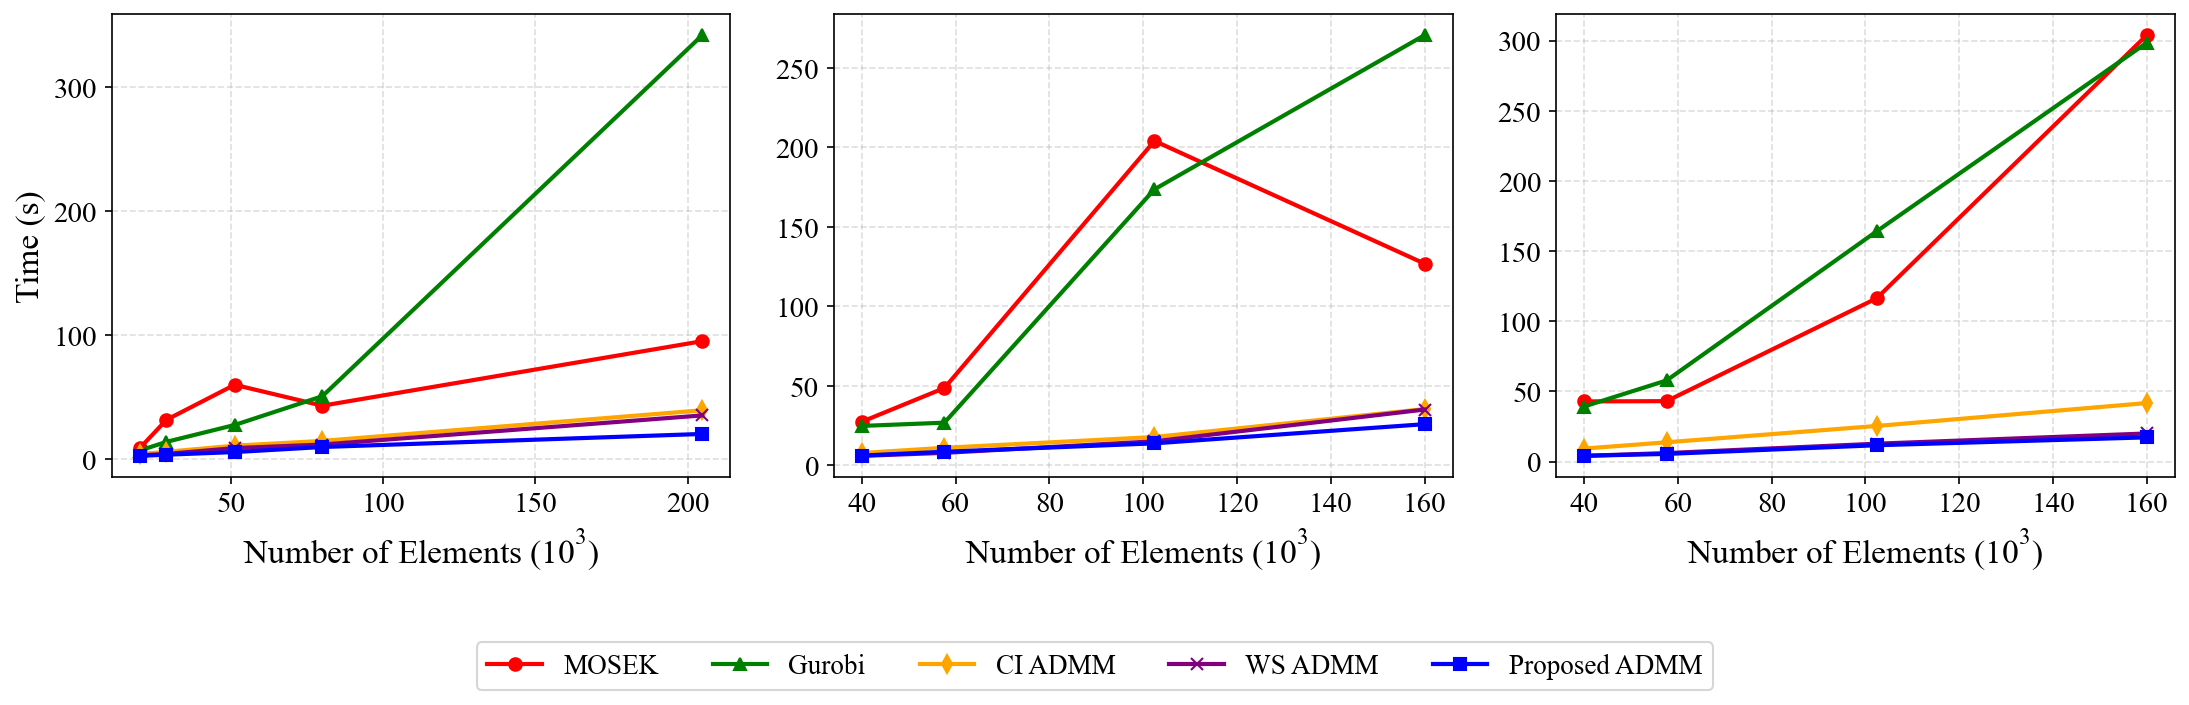
\includegraphics[width=0.95\textwidth]{figures/Res_To_Date/TC_ALL.png}
  \caption{Timing comparison of different ADMM implementations against IPM solvers in 2D benchmark problems using structured mesh (From left to right: Rigid platen, strip footing, vertical cut)}
  \label{fig:2DTimecomp}
\end{figure}
\begin{table}[htbp] 
\centering 
\caption{Performance enhancement achieved with warm-starting using adaptive refined mesh} 
\label{tab:2DWS_AMR} 
 
\begin{tabular}{@{}C{2.1cm}C{1.8cm}C{1.8cm}C{2cm}C{1.5cm}C{1.6cm}C{2.1cm}C{1.6cm}@{}} 
\toprule 
\textbf{Problem type} &
\multicolumn{2}{c}{\textbf{Problem size}} & 
\textbf{Warm starting} & 
\textbf{Solve time (s)} & 
\textbf{Iterations} & 
\textbf{Load multiplier} & 
\textbf{Speedup} 
\tabularnewline 
\cmidrule(lr){2-3} 
& 
\textbf{$N_{\mathrm{elem}}(\times 10^3)$} & 
\textbf{$N_{\mathrm{var}}(\times 10^6)$} & 
& 
& 
& 
& 
\tabularnewline 
\midrule 
 
\multirow{2}{*}{Rigid Platen} 
& \multirow{2}{*}{362.49} 
& \multirow{2}{*}{3.26} 
& Yes & 52.24 & 400 & 2.42681 & \multirow{2}{*}{16\%} \tabularnewline 
& & & No  & 61.91 & 460 & 2.42689 & \tabularnewline 
 
\addlinespace 
 
\multirow{2}{*}{Strip Footing} 
& \multirow{2}{*}{553.50} 
& \multirow{2}{*}{4.98} 
& Yes & 75.15 & 400 & 5.13648 & \multirow{2}{*}{40\%} \tabularnewline 
& & & No  & 125.35 & 620 & 5.13668 & \tabularnewline 
 
\addlinespace 
 
\multirow{2}{*}{Vertical Cut} 
& \multirow{2}{*}{452.23} 
& \multirow{2}{*}{4.07} 
& Yes & 77.56 & 460 & 3.77522 & \multirow{2}{*}{30\%} \tabularnewline 
& & & No  & 110.90 & 660 & 3.77549 & \tabularnewline 
 
\bottomrule 
\end{tabular} 
 
\vspace{0.5em} 
\end{table}


\subsection{3D Benchmark Problems}

\subsubsection{Rigid Platen Problem}
\paragraph{Problem setup} 


This example considers the 3D compression of a von Mises soil block between two rigid platens, as illustrated in Figure~\ref{fig:3D2PR_CS}. The soil domain has dimensions $L \times L \times 0.5L$. The soil is assumed to obey the von-Mises yield criterion. We exploit symmetry on the lower, frontal and diagonal boundaries, while the upper rigid platen is subjected to a vertical live load $F_{\mathrm{live}}$. The soil-platen interfaces are taken to be fully rough. The remaining right boundary is left free. By exploiting symmetry, only one sixteenth of the model needs to be analysed.

\begin{figure}[htbp]
  \centering
  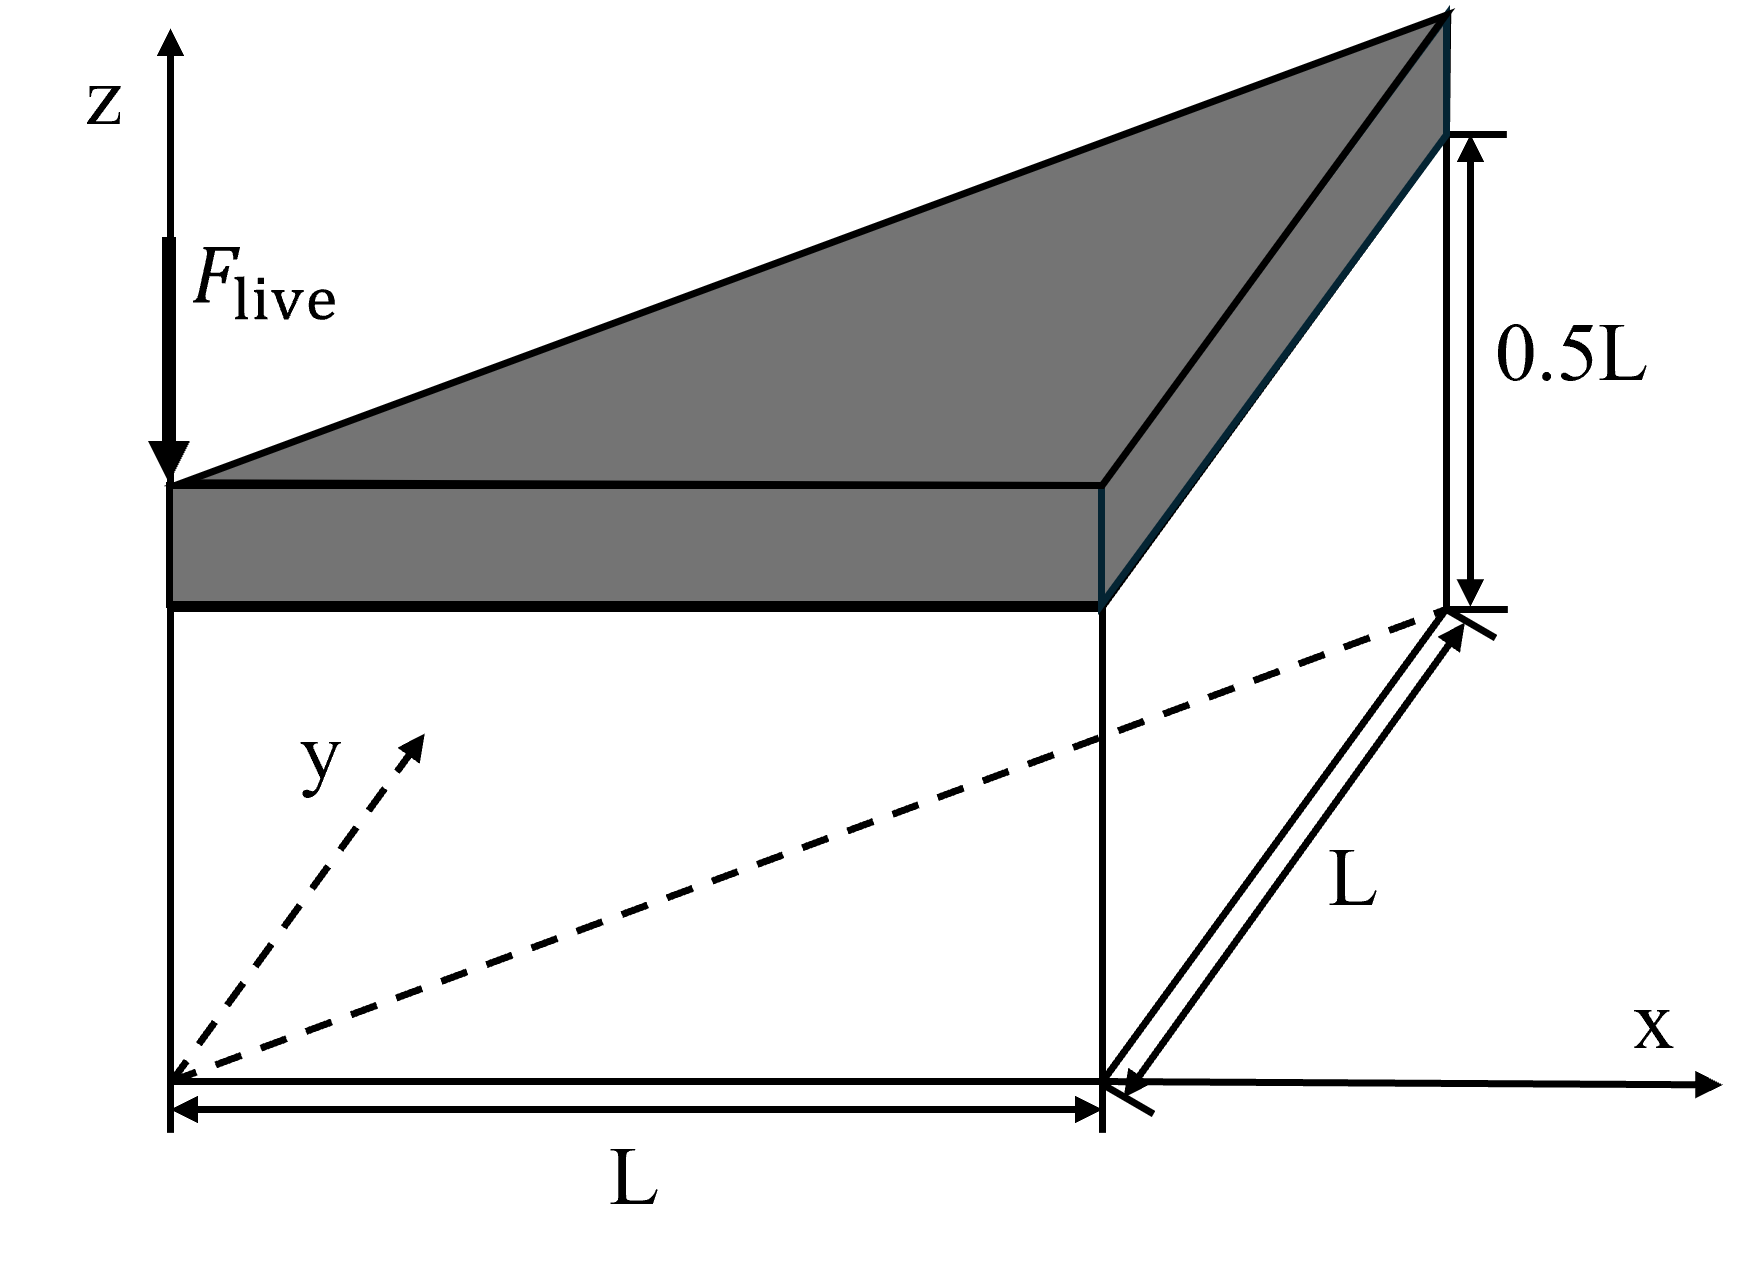
\includegraphics[width=0.44\textwidth]{figures/Res_To_Date/3D2PR_config.png}
  \hfill
  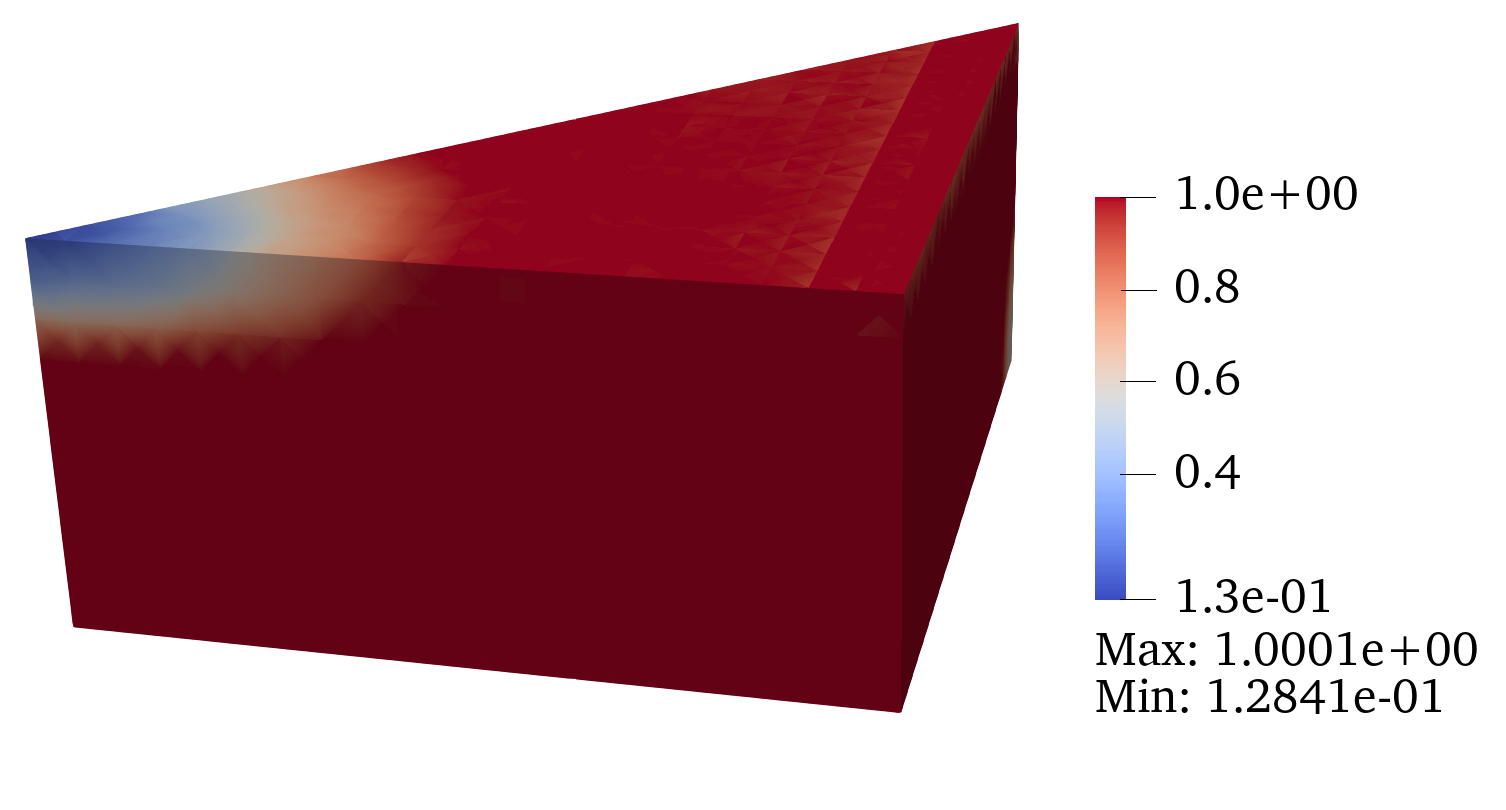
\includegraphics[width=0.55\textwidth]{figures/Res_To_Date/3D2PR_solution.png}
  \caption{3D rigid platen problem. \textbf{Left}: physical configuration; \textbf{Right}: solution of the yield function using a structured mesh}
  \label{fig:3D2PR_CS}
\end{figure}

\paragraph{Benchmark comparison using structured mesh} 

\begin{table}[htbp]
\centering
\caption{Solver performance comparison on the 3D rigid platen benchmark for different mesh discretizations}
\label{tab:3D2PR_table}

\begin{tabular}{@{}C{1.7cm}C{1.7cm}C{1.5cm}C{2.0cm}C{2.3cm}C{2.3cm}C{2.3cm}@{}}
\toprule
\multicolumn{2}{c}{\textbf{Problem size}} &
\textbf{Solver} &
\textbf{Solve time (s)} &
\textbf{Collapse multiplier} &
\textbf{Iterations} &
\textbf{Time-per-iter (s)}
\tabularnewline

\cmidrule(lr){1-2}

\textbf{$N_{\mathrm{elem}}(\times 10^3)$} &
\textbf{$N_{\mathrm{var}}(\times 10^6)$} &
&
&
&
&
\tabularnewline

\midrule

\multirow{3}{*}{6}
& \multirow{3}{*}{0.148}
& MOSEK		& 8.84	& 2.08904 & 24 & 0.37 \tabularnewline
& & Gurobi 	& 10.15  	& 2.08905 & 17 & 0.60 \tabularnewline
& & ADMM 	& 4.33 	& 2.08844 & 220 & 0.019 \tabularnewline

\addlinespace

\multirow{3}{*}{24.6}
& \multirow{3}{*}{0.589}
& MOSEK  		& 96.63	& 2.09546 & 33 & 2.93 \tabularnewline
& & Gurobi	& 147.24	& 2.09546 & 16 & 9.20\tabularnewline
& & ADMM   	& 22.33 	& 2.09526 & 220 & 0.10\tabularnewline

\addlinespace

\multirow{3}{*}{48}
& \multirow{3}{*}{1.152}
& MOSEK  & 371.2 & 2.09755 & 39 & 9.52 \tabularnewline
& & Gurobi & 618.31 & 2.09755 & 17 & 36.37 \tabularnewline
& & ADMM   & 61.99 & 2.09708 & 180 & 0.34\tabularnewline

\bottomrule
\end{tabular}

\vspace{0.5em}
\end{table}

Table~\ref{tab:3D2PR_table} shows that our solver still yields a speedup, from $2.04\times$ to $5.99\times$ compared with MOSEK in 3D FELA problems. Speedup is achieved in both linear and linear elements, with the largest speedup of $5.99\times$ achieved at the largest linear case. It should be noted however, the sparsity pattern of the 3D problem differs from that of the 2D problems, thereby incurring a substantial increase in the number of fill-ins in direct factorization, which limited the maximum problem size we can explore.

\subsubsection{Square Footing Problem}

\paragraph{Problem setup}
Similar to the 2D strip footing problem, the square footing problem considers a rigid footing resting on the surface of a soil body. By exploiting symmetry, only one eighth of the full domain is modelled. Symmetry boundary conditions are imposed on the diagonal plane and the frontal plane. The rigid footing is located at the top-left corner of the computational domain, corresponding to the symmetric portion of the full square footing. The footing side length is set to one fifth of the characteristic length of the soil body, i.e. $L$ for a soil domain of characteristic length $5L$. The bottom boundary and the far-field lateral boundary on the right-hand side are fixed, while the remaining external boundaries are left free unless constrained by symmetry or footing contact conditions.

No analytical lower-bound solution appears to be available for the square or rectangular footing problem. However, da Silva and Salgado~\cite{daSilva_2020, Salgado_2004} investigated this problem with Tresca criterion using FELA and with linear stress elements. Salgado~\cite{Salgado_2004} reported a lower-bound solution of 5.523 using a tailored mesh with thin elements near the footing edge, whereas da Silva~\cite{daSilva_2020} obtained a lower-bound solution of 5.625 on a very fine structured mesh.

\begin{figure}[htbp]
  \centering
  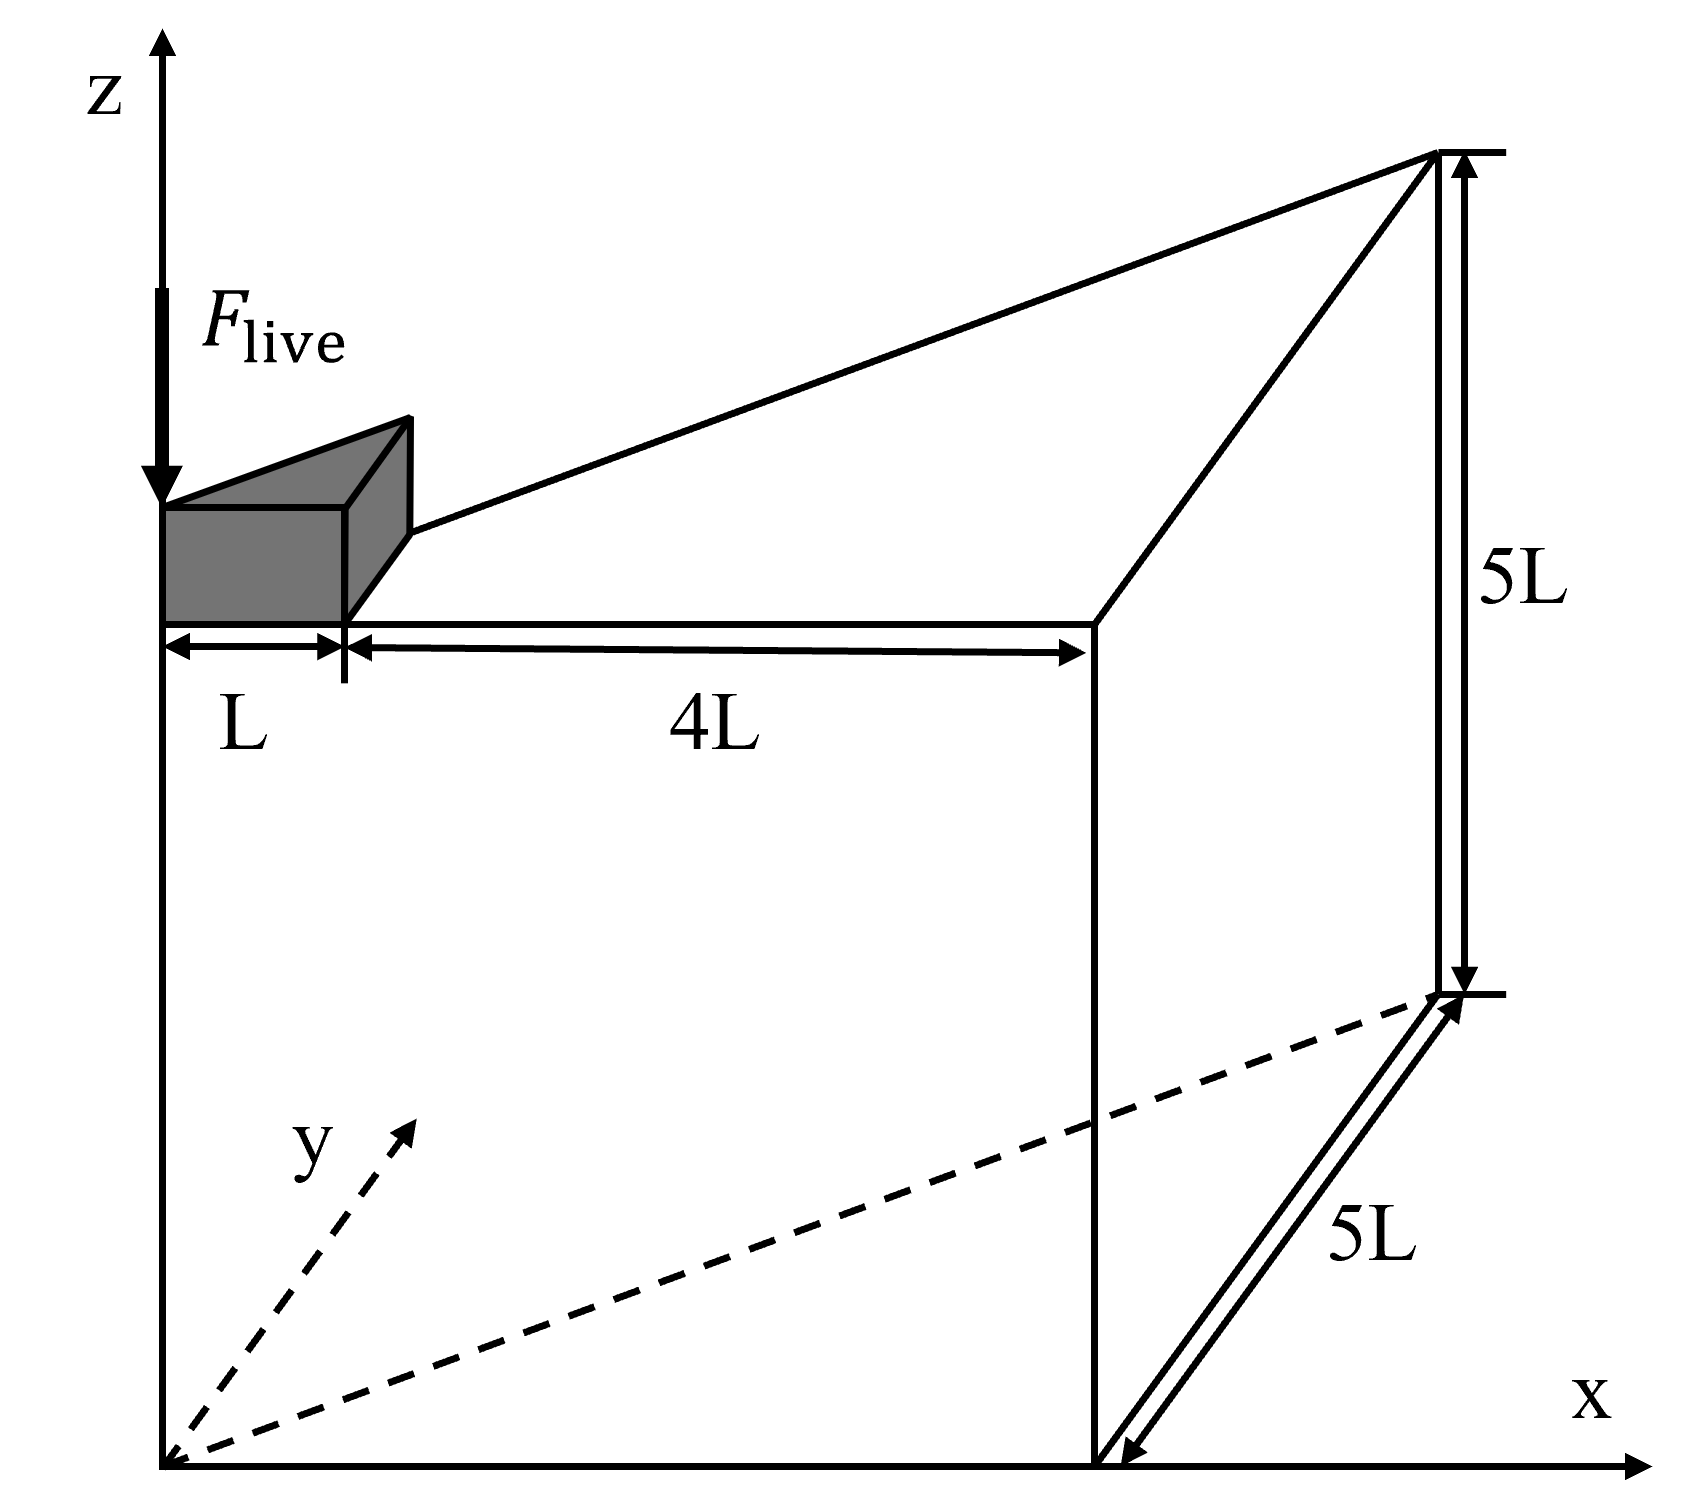
\includegraphics[width=0.46\textwidth]{figures/Res_To_Date/3DSF_config.png}
  \hfill
  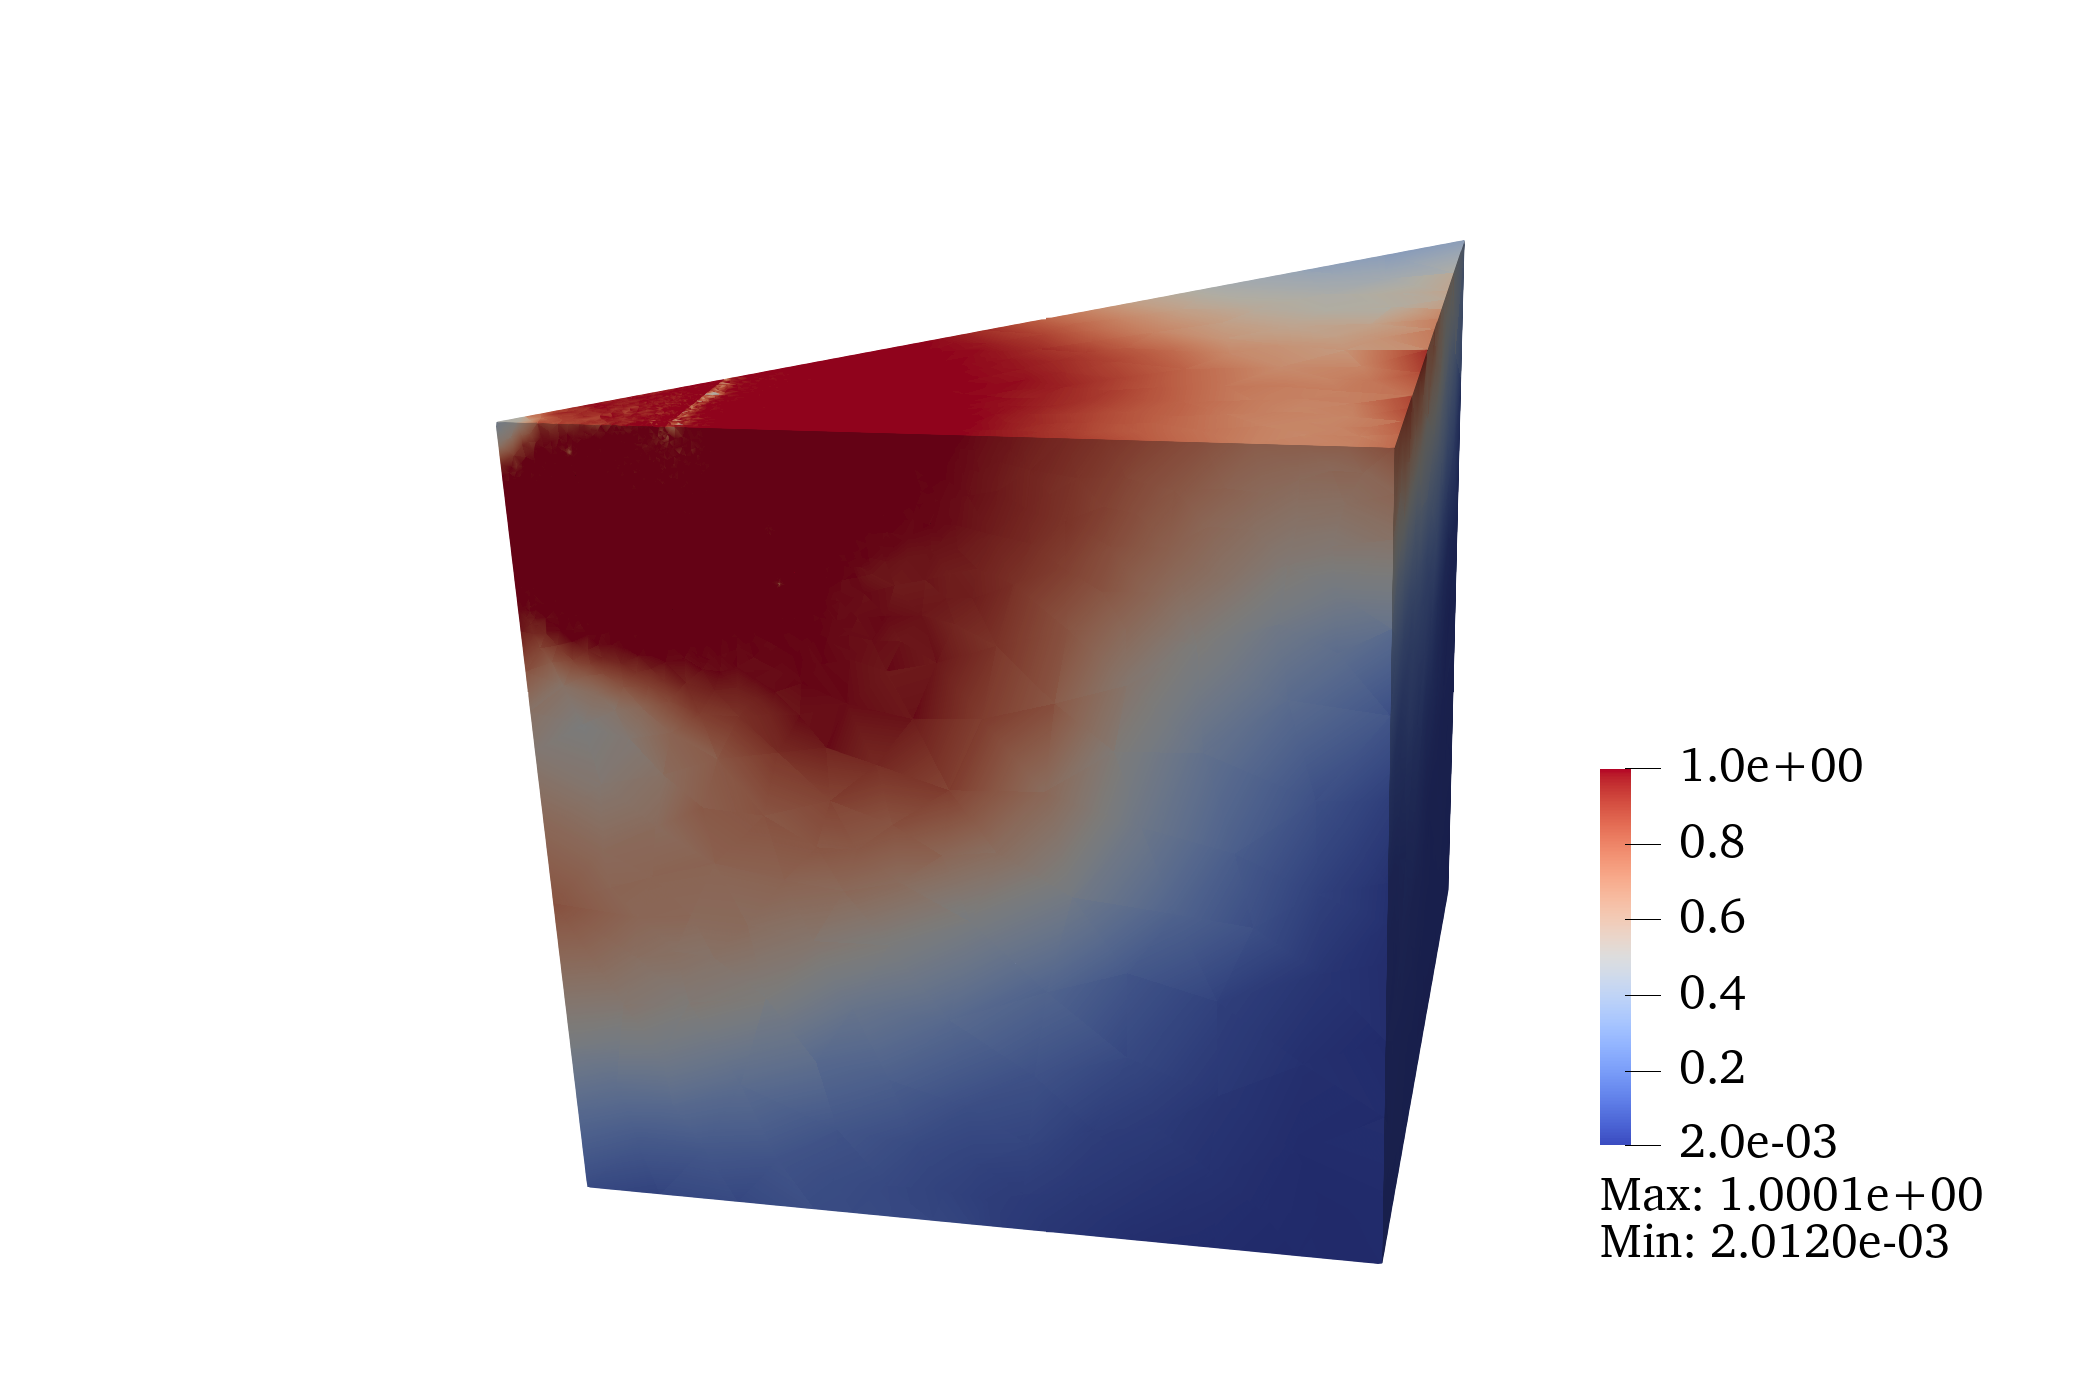
\includegraphics[width=0.53\textwidth]{figures/Res_To_Date/3DSF_solution_AMR.png}
  \caption{3D square footing problem. \textbf{Left}: physical configuration; \textbf{Right}: solution of the yield function using a refined quadratic mesh}
  \label{fig:3DSF_CS}
\end{figure}


\paragraph{Benchmark comparison using structured mesh}

The performance of the proposed 3D ADMM solver is first assessed on structured meshes and compared against MOSEK. The results are summarized in Table~\ref{tab:3DSF_table}. Similar to the previous benchmarks, both the time-to-solution and the computed collapse multiplier are reported.

\begin{table}[htbp]
\centering
\caption{Solver performance comparison on the 3D square footing benchmark for different mesh discretizations}
\label{tab:3DSF_table}

\begin{tabular}{@{}C{1.7cm}C{1.7cm}C{1.5cm}C{2.0cm}C{2.3cm}C{2.3cm}C{2.3cm}@{}}
\toprule
\multicolumn{2}{c}{\textbf{Problem size}} &
\textbf{Solver} &
\textbf{Solve time (s)} &
\textbf{Collapse multiplier} &
\textbf{Iterations} &
\textbf{Time-per-iter (s)}
\tabularnewline

\cmidrule(lr){1-2}

\textbf{$N_{\mathrm{elem}}(\times 10^3)$} &
\textbf{$N_{\mathrm{var}}(\times 10^6)$} &
&
&
&
&
\tabularnewline

\midrule

\multirow{3}{*}{12}
& \multirow{3}{*}{0.288}
& MOSEK  		& 20.87	& 5.22710 & 27	&  0.77\tabularnewline
& & Gurobi 	& 31.93	& 5.22716 & 16 	&  1.99\tabularnewline
& & ADMM   	& 17.65	& 5.22694 & 420 & 0.042 \tabularnewline

\addlinespace

\multirow{3}{*}{96}
& \multirow{3}{*}{2.304}
& MOSEK  & 937.53 & 5.36728 & 32  & 29.29  \tabularnewline
& & Gurobi$^{\dagger}$ &  --    & --      & -- & $\approx$ 200 \tabularnewline
& & ADMM   & 538.21 & 5.36173 & 540 & 0.99 \tabularnewline

\bottomrule
\end{tabular}

\begin{minipage}{0.98\linewidth}
\footnotesize
$^{\dagger}$ Gurobi did not complete the larger problem. The reported estimated time per iteration was approximately \(200\,\mathrm{s}\); therefore, the run was terminated due to the excessive computational time.

\end{minipage}

\vspace{0.5em}
\end{table}




Table~\ref{tab:3DSF_table} shows that across all tested cases, the relative discrepancy between the two solvers remains small, confirming that the proposed ADMM can recover high-quality LB solutions for this 3D benchmark. Refining the linear mesh to $96\times10^3$ elements increases the collapse multiplier to about $5.36$. This trend is consistent with the expected convergence of lower-bound FELA solutions under mesh refinement.

In terms of computational performance, the ADMM solver remains faster than MOSEK, with speedups ranging from approximately $1.27\times$ to $2.61\times$. These speedups are more modest than those observed in the 2D strip footing benchmark and in the 3D rigid platen problem. This is because the square footing problem produces a more demanding three-dimensional KKT system, for which sparse direct factorization introduces substantially more fill-in. Consequently, the cost of storing and applying the factorized matrices becomes a dominant part of the total solution time. The benchmark therefore highlights both the robustness of the proposed solver and the memory-related scalability bottleneck of the current direct-solve implementation in 3D.

\paragraph{Adaptive mesh refinement}

Here we demonstrate the ability of our methodology to obtain an accurate LB solution in 3D. We were able to obtain an accurate LB solution of $\beta = 5.40200$. This solution is obtained with 8 adaptive mesh refinements with 0.18 million linear stress elements, and the adaptive mesh obtained is shown in Figure~\ref{fig:3DSF_AMR_SOL}.

\begin{figure}
\centering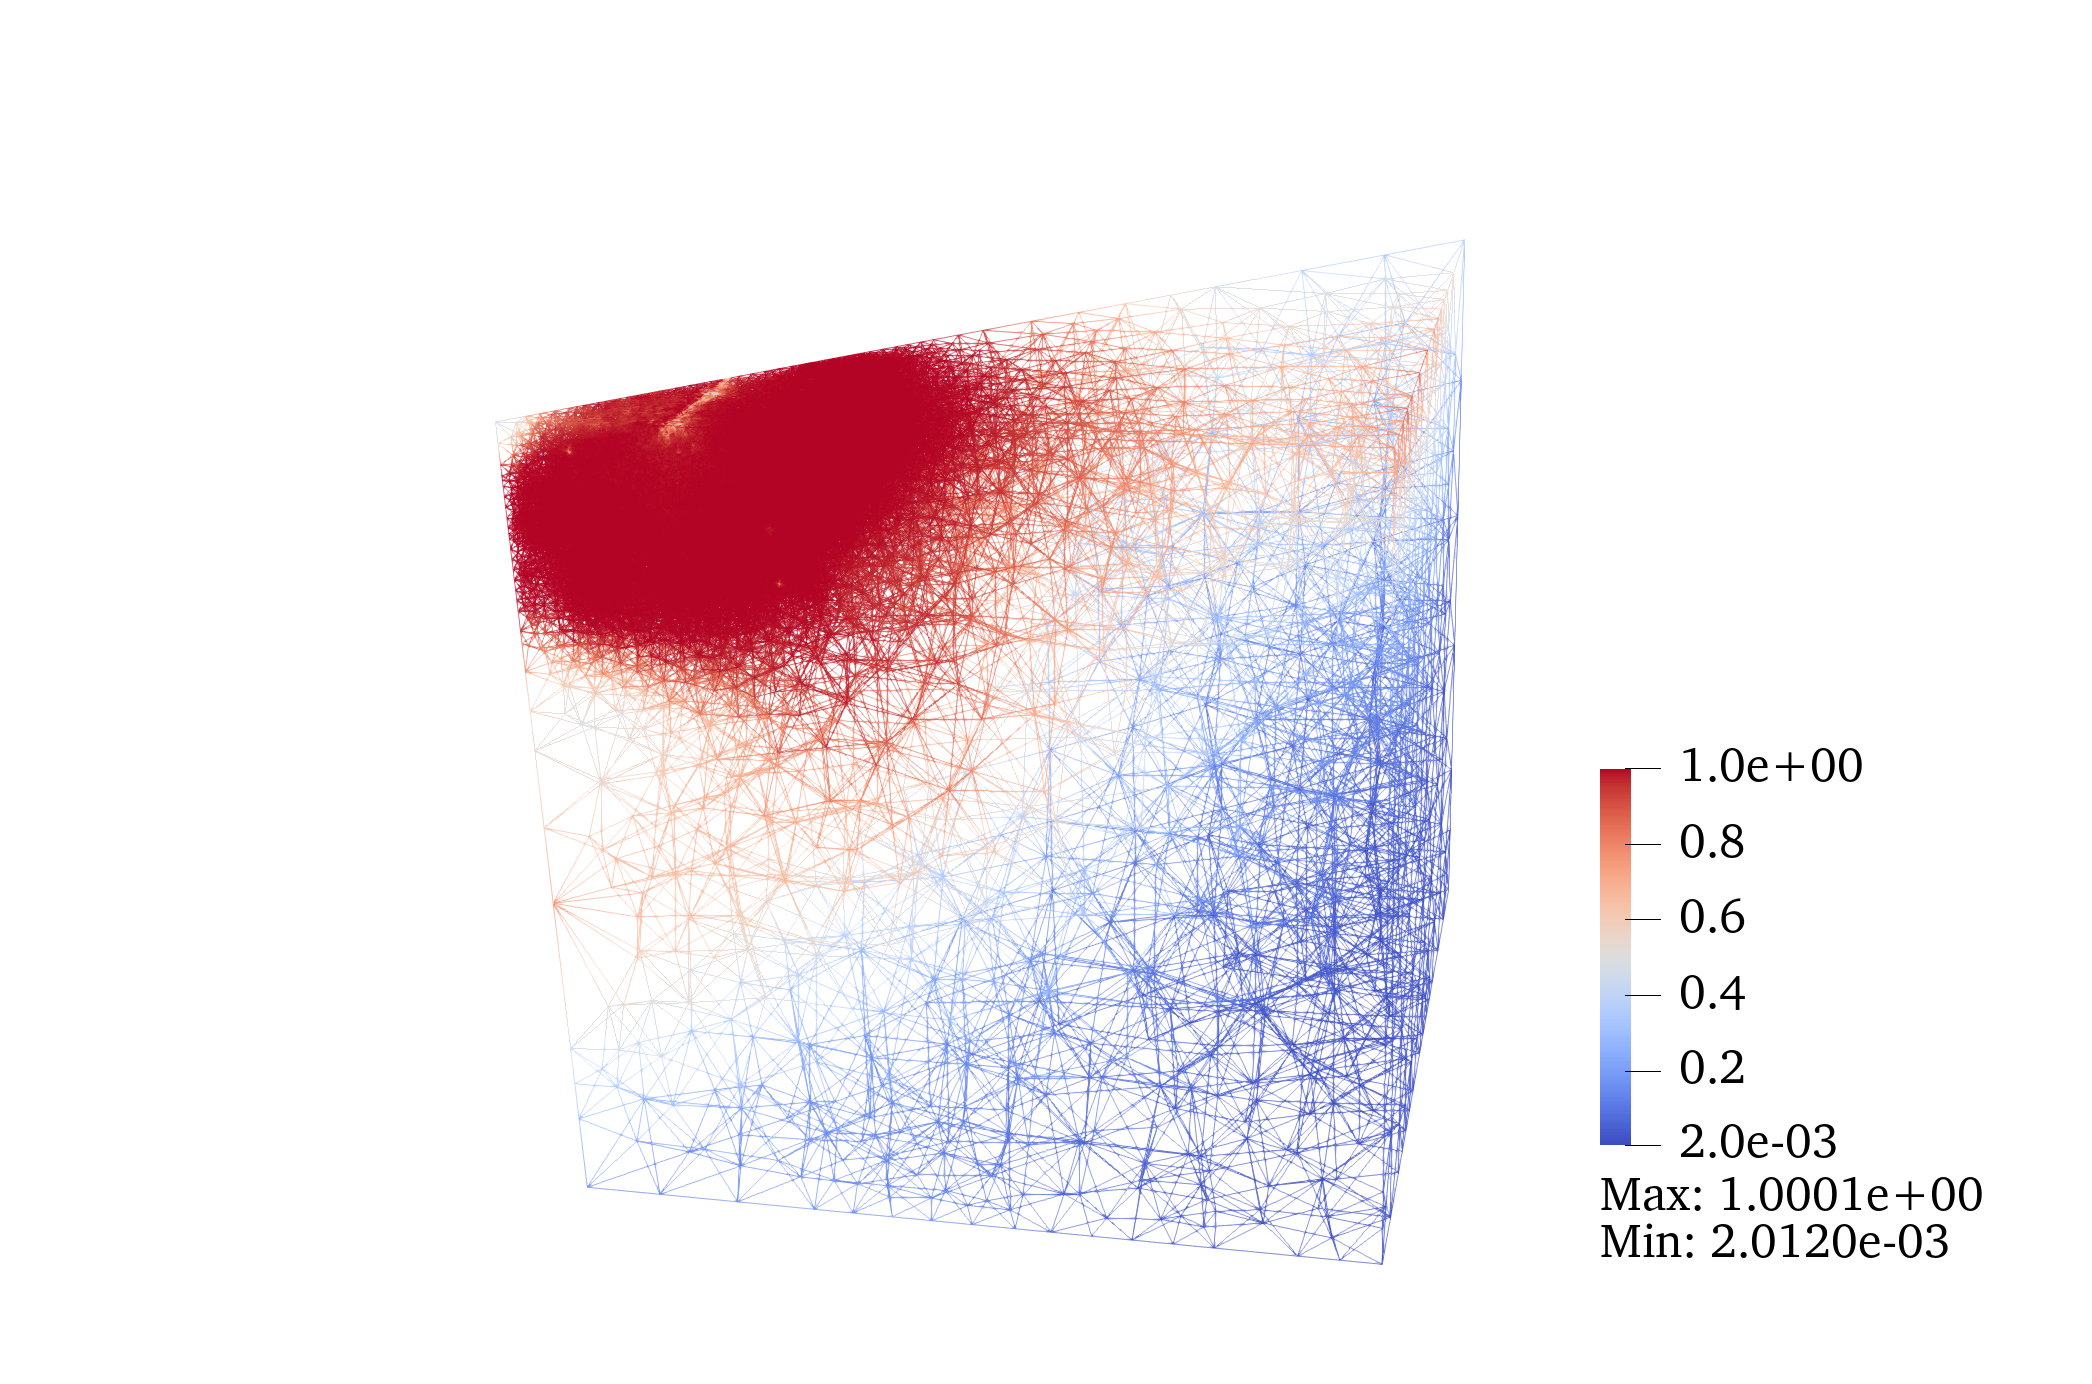
\includegraphics[width=0.8\textwidth]{figures/Res_To_Date/AMR_A1000.png} 
\caption{AMR result of the square footing problem}
\label{fig:3DSF_AMR_SOL}
\end{figure}

The AMR result demonstrates that the proposed framework can be extended to challenging three-dimensional FELA problems and can automatically concentrate resolution in the critical yielding region as shown in the upper left corner of the soil body in Figure~\ref{fig:3DSF_AMR_SOL}. Nevertheless, the process was stopped after 8 refinements because the excessive fill-in introduced by sparse direct factorization exhausted the available GPU device memory. This limitation arises from the direct factorization-solve routine, and could potentially be alleviated in larger 3D problems by adopting an indirect, matrix-free linear solver.

\subsubsection{Vertical Cut Problem}

\paragraph{Problem Setup}

In 3D, the geometry of the cut is characterized by the aspect ratio $H/B$, where $H$ denotes the depth of the cut and $B$ denotes its width. Unless otherwise stated, we consider the case $H/B=5$, with $H=1$, $B=0.2$, and $L=2$, so that the computational domain is sufficiently large to contain the potential failure mechanism. Similar to its 2D counterpart, the soil is modelled as a von Mises material subjected to a uniform body force representing the live load. The vertical cut surface and the top surface are taken as free boundaries; the front and back diagonal surfaces are treated as symmetry planes; and the right and bottom surfaces are fixed. The physical configuration is illustrated in Figure~\ref{fig:3DVC_CS}. Exploiting symmetry, only one quarter of the soil domain is modelled.


\begin{figure}[htbp]
  \centering
  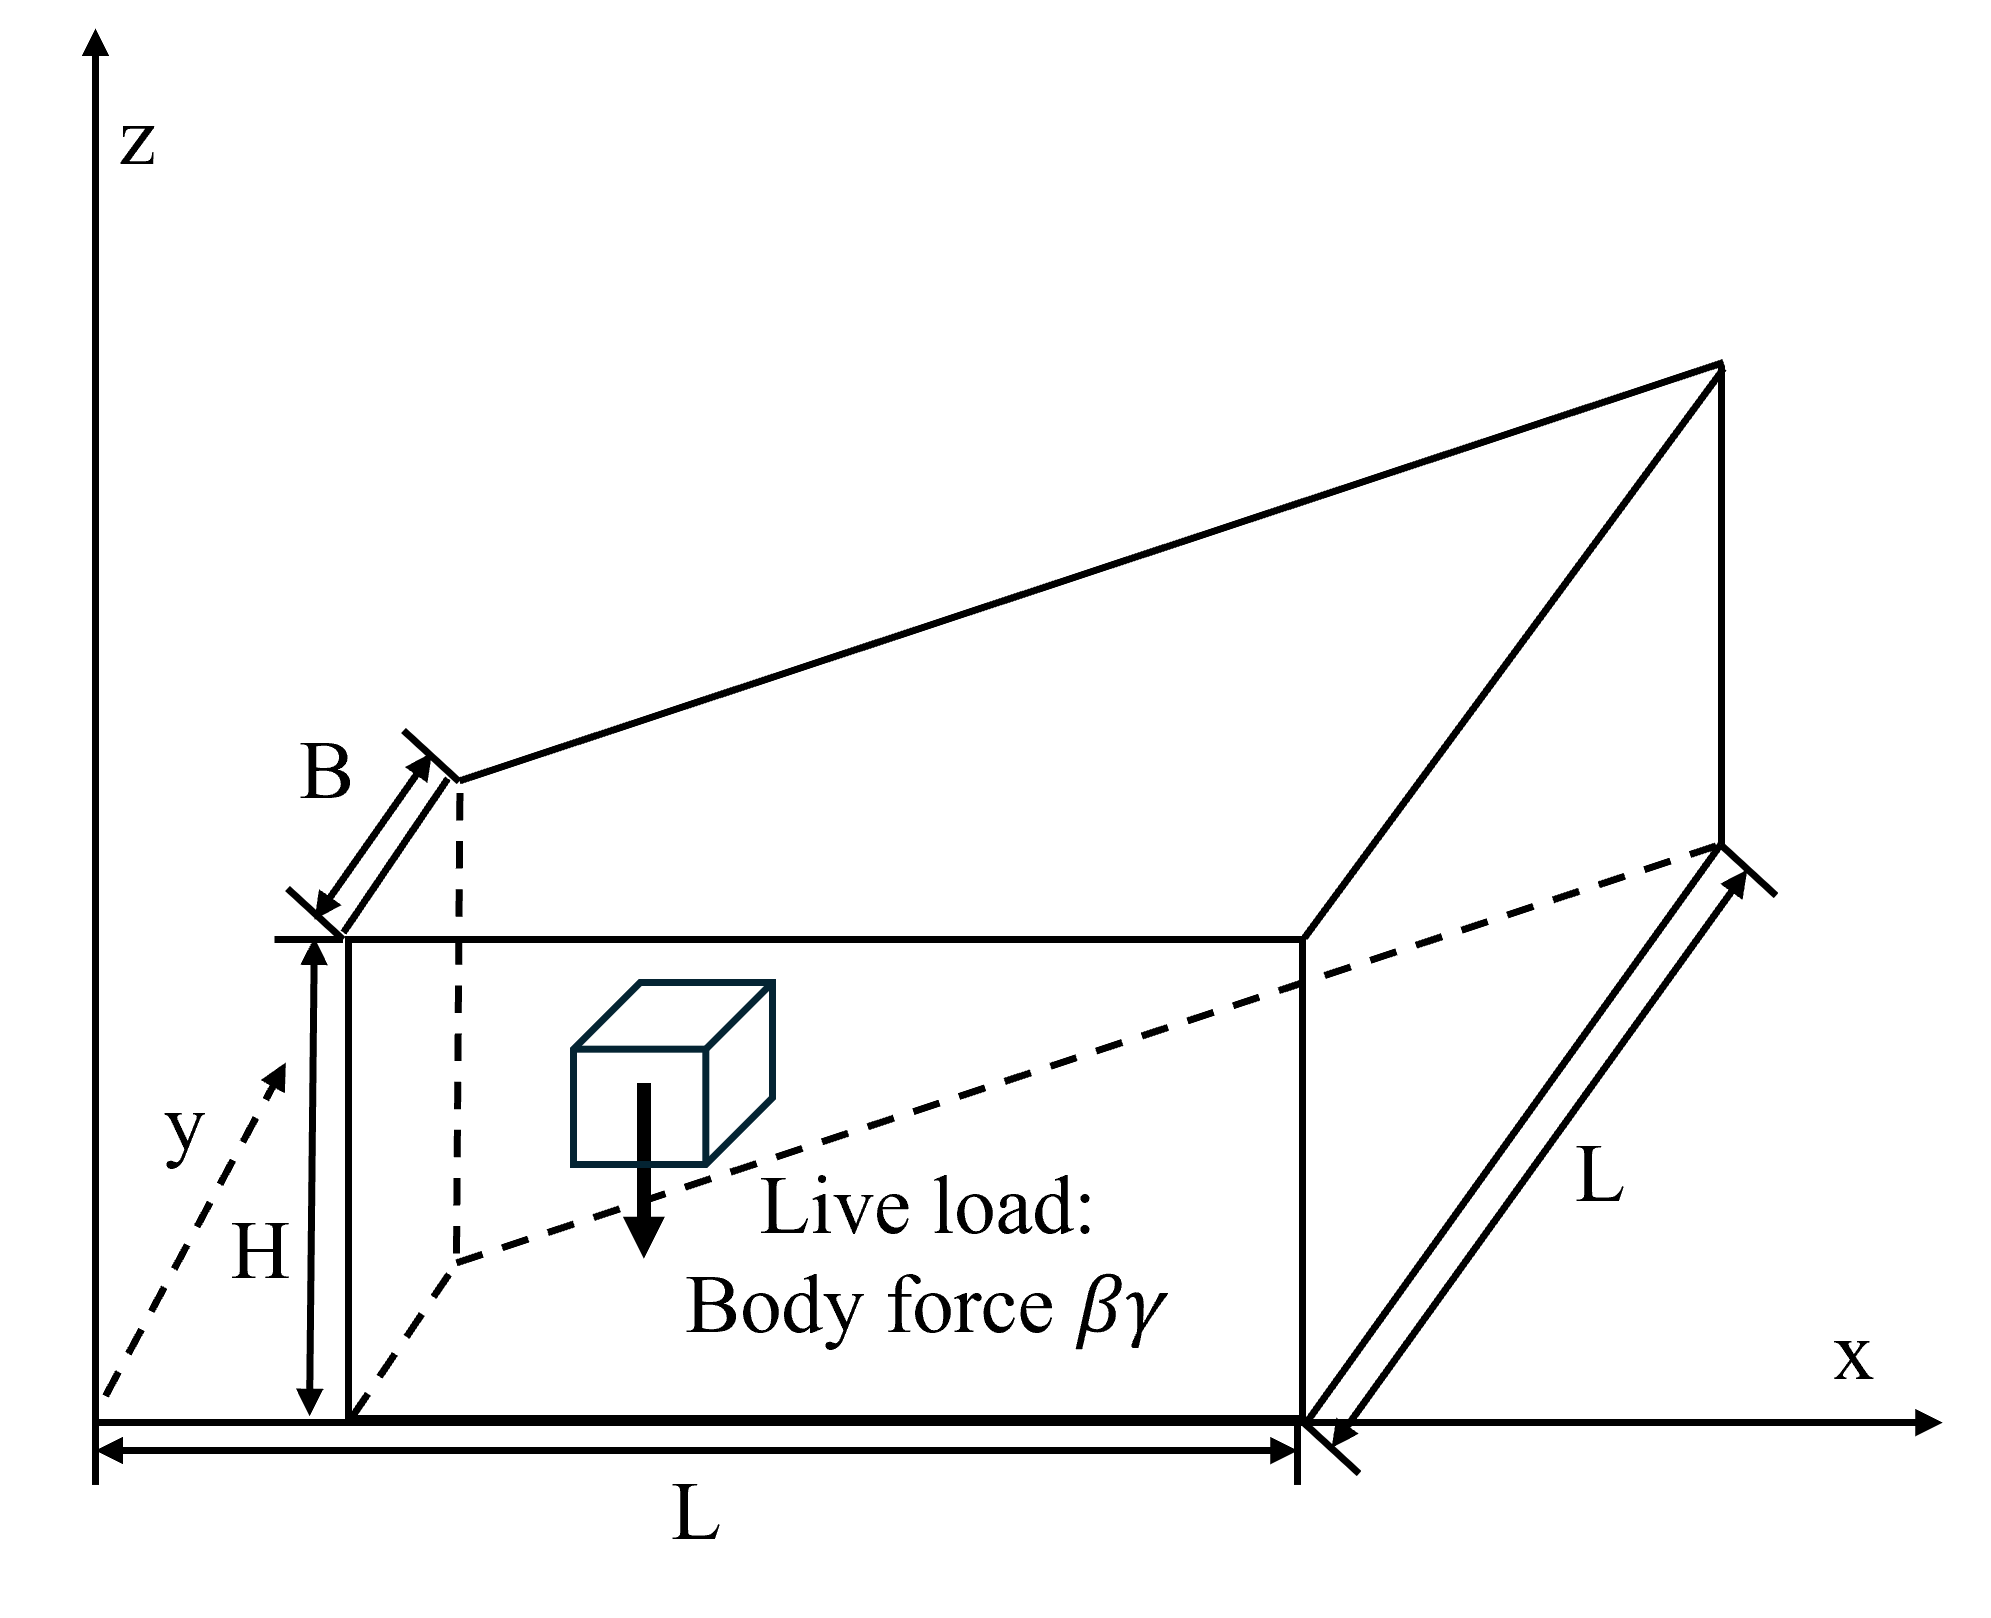
\includegraphics[width=0.44\textwidth]{figures/Res_To_Date/3DVC_config.png}
  \hfill
  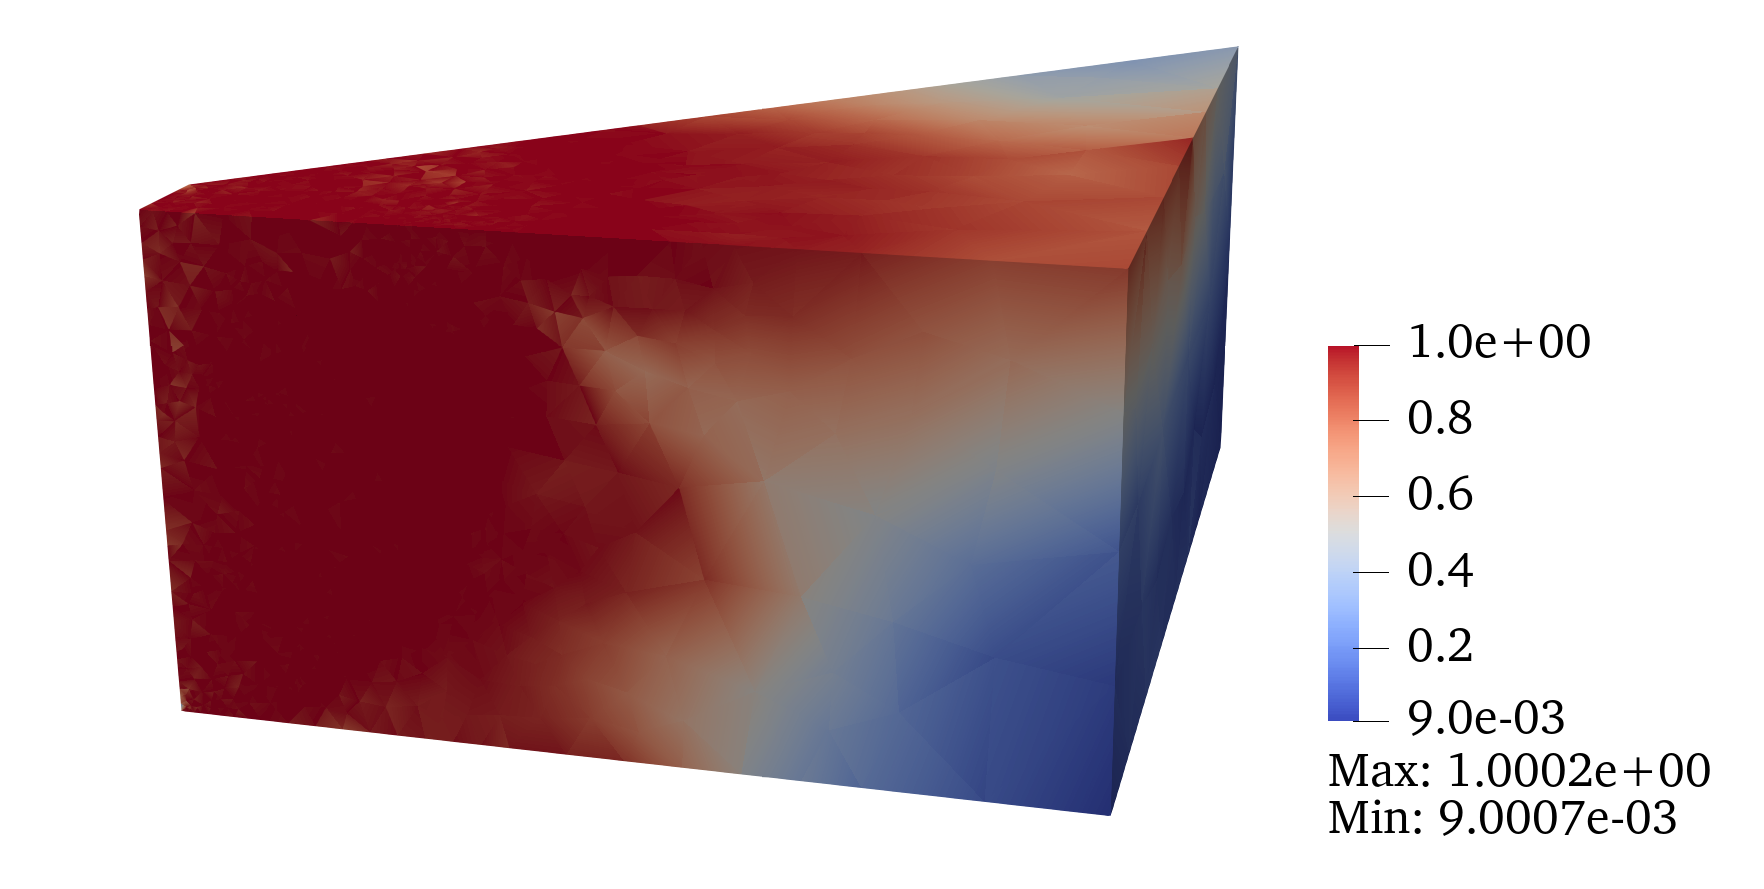
\includegraphics[width=0.55\textwidth]{figures/Res_To_Date/3DVC_solution.png}
  \caption{3D vertical cut problem. \textbf{Left}: physical configuration; \textbf{Right}: solution of the yield function using a refined mesh}
  \label{fig:3DVC_CS}
\end{figure}


\paragraph{Adaptive Mesh Solution}
Adaptive mesh refinement enables the failure mechanism of the vertical cut to be resolved in greater detail. Figure~\ref{fig:3DVC_AMR} presents the corresponding adaptive mesh in wireframe form. For the formulation employing linear stress elements, the best load multiplier obtained is $\beta = 6.55712$. The failure zone is clearly captured by the highly refined red region adjacent to the vertical excavation.

\begin{figure}[htbp]
  \centering
  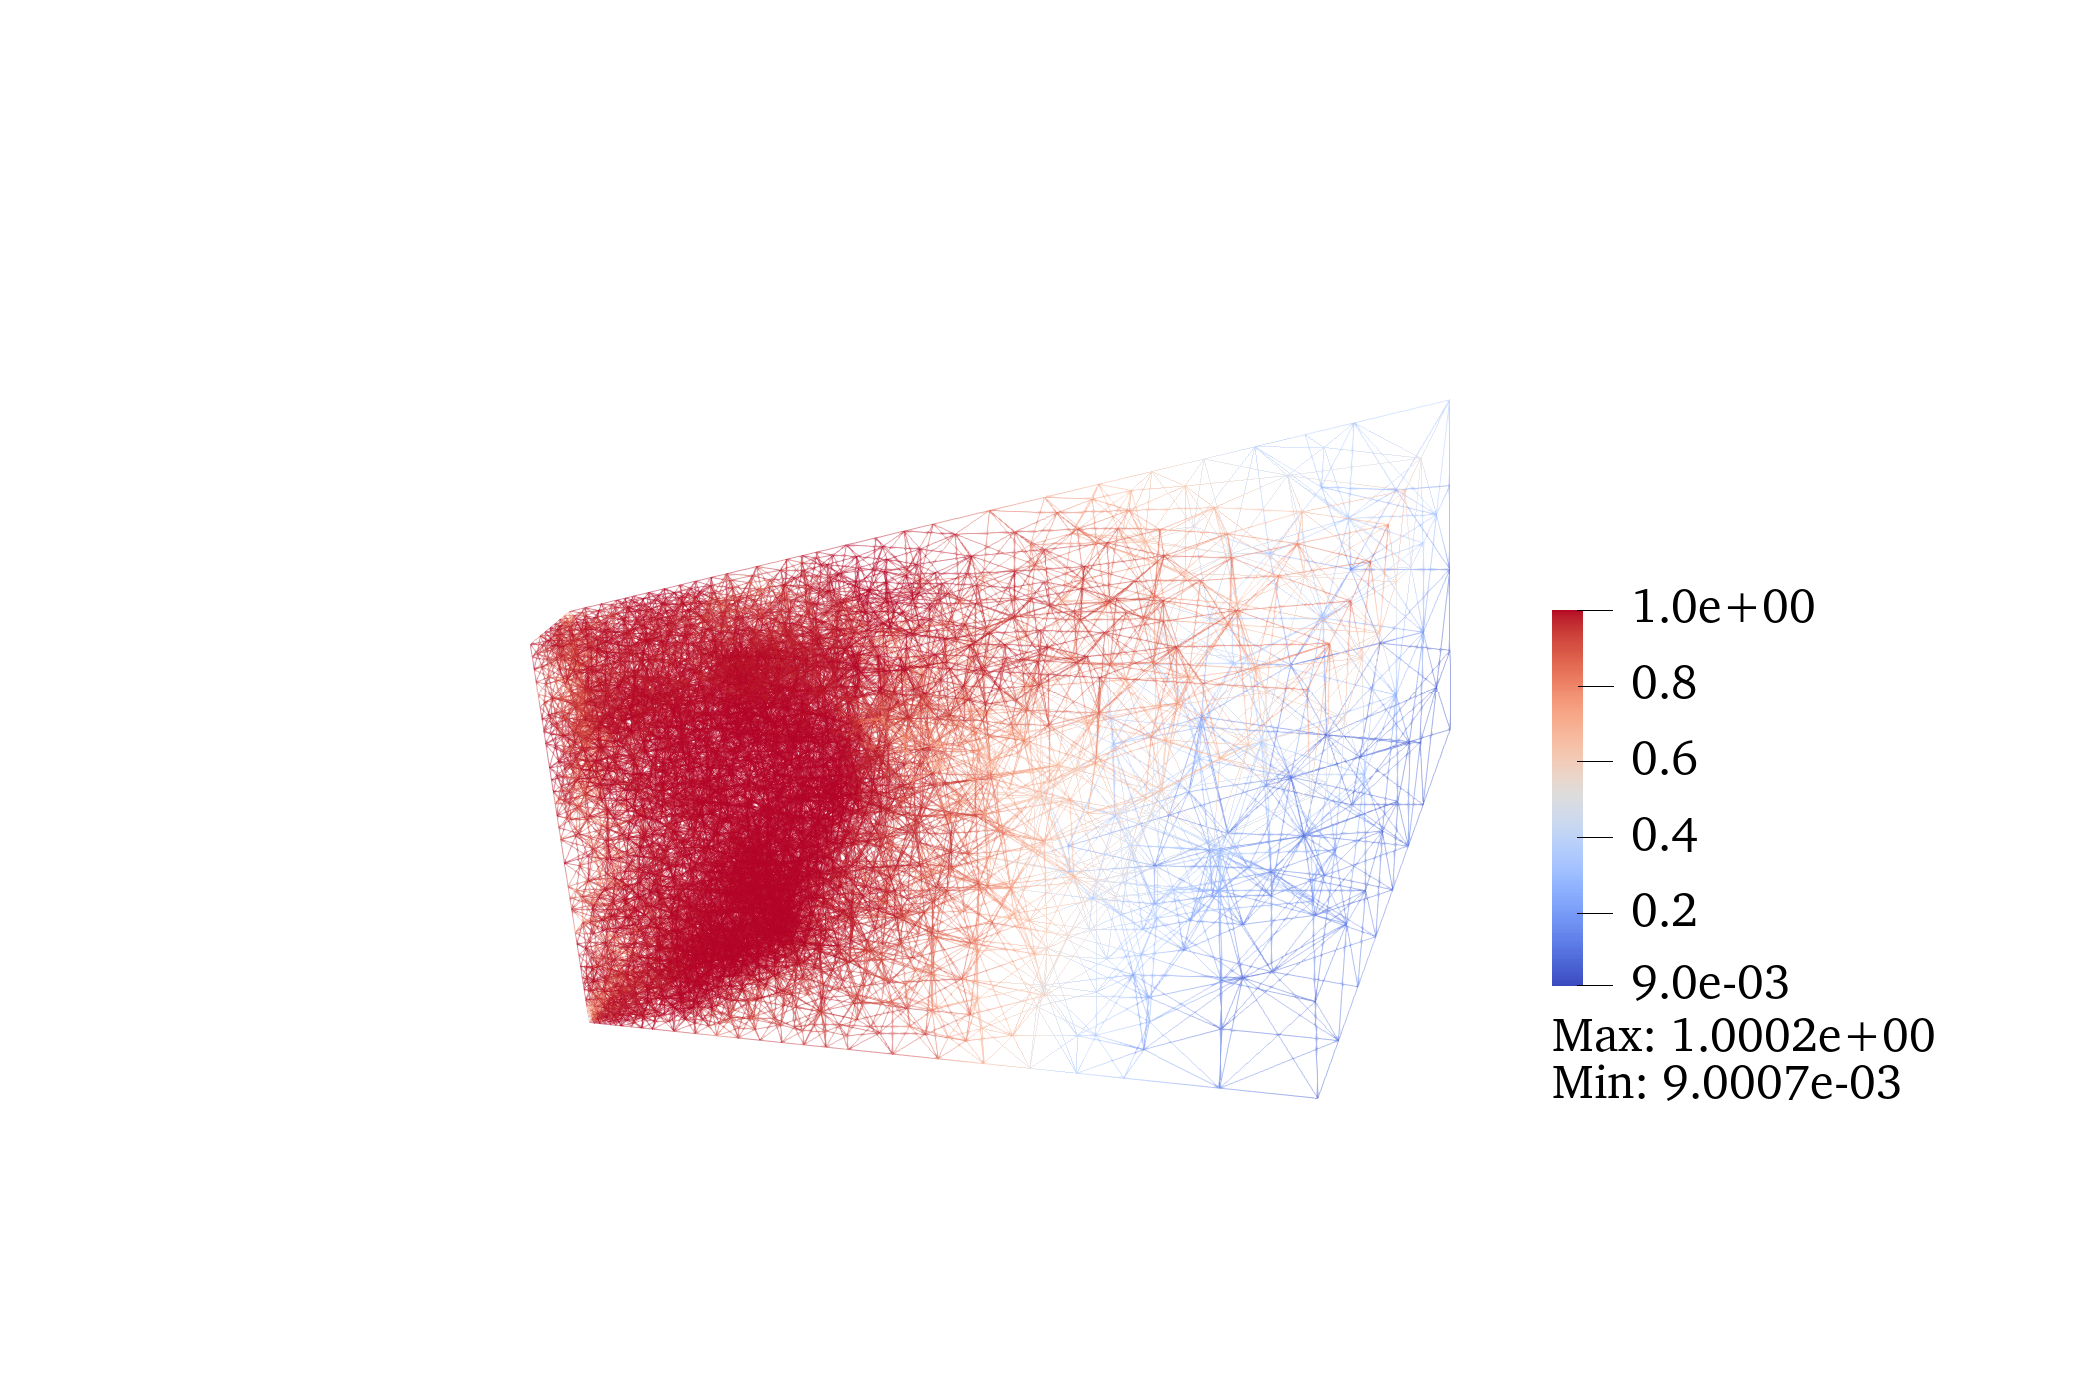
\includegraphics[width=0.8\textwidth]{figures/Res_To_Date/3DVC_AMR_Mesh.png}
  \caption{AMR result of the vertical cut problem in 3D}
  \label{fig:3DVC_AMR}
\end{figure}
\subsubsection{Discussion}

As in the 2D examples, the proposed ADMM solver remains computationally competitive in the 3D benchmarks. Although the speedup over the IPM solvers is generally less pronounced than in 2D, the computational cost per ADMM iteration remains substantially lower than that of an IPM iteration. Moreover, with warm-starting and active-cone identification, the number of ADMM iterations varies only moderately as the problem size increases.

The reduced speedup observed in 3D is not primarily caused by a deterioration of the ADMM iteration itself. Instead, the dominant computational cost shifts increasingly toward the sparse linear algebra, particularly numerical factorization and repeated triangular solves. This effect is much more pronounced in three-dimensional FELA because of the denser connectivity and greater fill-in generated during factorization. The underlying scalability implications are discussed in detail in Section~\ref{sec:3D_scalability}.

To further examine how the individual solver enhancements contribute to the overall performance in 3D, we consider the rigid platen benchmark with a structured mesh of 48,000 linear tetrahedral stress elements and approximately 1.15 million variables. A vanilla GPU-accelerated ADMM implementation already benefits from inexpensive repeated iterations through factorization reuse, while the proposed framework introduces additional mechanisms to improve convergence and reduce the cost of the underlying linear algebra. We therefore compare several solver configurations involving warm-starting (WS), active-cone identification (CI), augmented (AUG) and condensed linear-system formulations, and the alternative ellipsoidal projection strategy. The corresponding results are summarized in Table~\ref{tab:Ablation_table}.


\begin{table}[htbp]
\centering
\caption{Solver performance with different solver options}
\label{tab:Ablation_table}
\begin{tabular}{@{}p{3cm}p{1.8cm}p{1.6cm}p{2cm}p{2.5cm}p{1.4cm}@{}}
\toprule
\textbf{Solver options} & \textbf{Solve time (s)} & \textbf{Iterations} &  \textbf{Analysis time (s)} & \textbf{Factorization time (s)} & \textbf{$\beta$} \\
\midrule
\texttt{AUG + Projection} 	& 41.30  	& 140 	& 19.20 & 18.31 & 2.09477 \\
\texttt{AUG + WS + CI}    	& 61.99  	& 180	& 19.58 & 16.21 & 2.09708 \\
\texttt{AUG + CI}         	& 110.74	& 280 	& 19.82 & 16.01 & 2.09229 \\
\texttt{AUG + WS}         	& 98.34  	& 600 	& 19.96 & 16.09 & 2.09750 \\
\texttt{Condensed}        	& 352.05   & 440  	& 37.35 & 45.00 & 2.09749 \\

\bottomrule
\end{tabular}
\vspace{0.5em}
\end{table}

The individual effects of warm-starting and active-cone identification are evident from the comparison between AUG+WS, AUG+CI, and AUG+WS+CI. Warm-starting alone requires 600 iterations, whereas active-cone identification reduces this to 280 iterations, indicating that CI is particularly effective in accelerating the later stages of convergence. However, CI changes the entries of the system matrix and therefore introduces repeated numerical refactorizations. Consequently, despite the lower iteration count, AUG+CI requires 110.74s, compared with 98.34s for AUG+WS. Combining the two strategies provides a better balance between convergence acceleration and refactorization overhead, reducing the iteration count further to 180 and the total solution time to 61.99s.

The alternative ellipsoidal projection strategy provides a further reduction in computational cost for this particular 3D problem. Compared with AUG+WS+CI, the projection-based formulation reduces the number of iterations from 180 to 140 and the total solution time from 61.99s to 41.30s. However, this improvement is accompanied by a slightly larger discrepancy in the computed collapse multiplier, with $\beta=2.09477$ compared with $\beta=2.09708$ for AUG+WS+CI. Although the difference remains small, the AUG+WS+CI configuration provides a more consistent balance between computational efficiency and solution accuracy. For this reason, AUG+WS+CI is adopted as the default configuration in the remaining 3D benchmark comparisons.

The choice of linear-system formulation has an even stronger influence on the computational cost in 3D. The condensed formulation (with warm-starting and cone identification) requires 352.05s, substantially longer than the augmented configurations, and also incurs markedly larger analysis and factorization costs. Unlike the convergence enhancements discussed above, this difference originates primarily from the sparse linear algebra rather than from the number of ADMM iterations. Indeed, the condensed formulation converges in 440 iterations, fewer than the 600 iterations required by the AUG+WS configuration, yet still takes substantially longer to solve. Forming and factorizing the condensed system generates substantially more fill-in in the 3D problem, increasing both memory consumption and the cost of each repeated triangular solves. This observation motivates the more detailed discussion of the 3D direct-factorization bottleneck in Section~\ref{sec:3D_scalability}.

The use of adaptive mesh refinement also yields tighter lower-bound solutions and provides a more detailed representation of the localized failure region. However, in the present 3D implementation, further refinement is ultimately constrained by the memory demand of sparse direct factorization. This observation reinforces the need for more memory-scalable linear-solver strategies in large-scale 3D FELA.
